\documentclass[12pt]{beamer}
\usepackage{../Estilos/BeamerFC}
\usepackage{../Estilos/ColoresLatex}
\usepackage{courier}
\usepackage{listingsutf8}
\usepackage{listings}
\usepackage{xcolor}
\usepackage{textcomp}
\usepackage{color}
\definecolor{deepblue}{rgb}{0,0,0.5}
\definecolor{brown}{rgb}{0.59, 0.29, 0.0}
\definecolor{OliveGreen}{rgb}{0,0.25,0}
% \usepackage{minted}

\DeclareCaptionFont{white}{\color{white}}
\DeclareCaptionFormat{listing}{\colorbox{gray}{\parbox{0.98\textwidth}{#1#2#3}}}
\captionsetup[lstlisting]{format=listing,labelfont=white,textfont=white}
\renewcommand{\lstlistingname}{Código}


\definecolor{Code}{rgb}{0,0,0}
\definecolor{Keywords}{rgb}{255,0,0}
\definecolor{Strings}{rgb}{255,0,255}
\definecolor{Comments}{rgb}{0,0,255}
\definecolor{Numbers}{rgb}{255,128,0}

\makeatletter

\newif\iffirstchar\firstchartrue
\newif\ifstartedbyadigit
\newif\ifprecededbyequalsign

\newcommand\processletter
{%
  \ifnum\lst@mode=\lst@Pmode%
    \iffirstchar%
        \global\startedbyadigitfalse%
      \fi
      \global\firstcharfalse%
    \fi
}

\newcommand\processdigit
{%
  \ifnum\lst@mode=\lst@Pmode%
      \iffirstchar%
        \global\startedbyadigittrue%
      \fi
      \global\firstcharfalse%
  \fi
}

\lst@AddToHook{OutputOther}%
{%
  \lst@IfLastOtherOneOf{=}
    {\global\precededbyequalsigntrue}
    {}%
}

\lst@AddToHook{Output}%
{%
  \ifprecededbyequalsign%
      \ifstartedbyadigit%
        \def\lst@thestyle{\color{orange}}%
      \fi
    \fi
  \global\firstchartrue%
  \global\startedbyadigitfalse%
  \global\precededbyequalsignfalse%
}

\lstset{ 
language=Python,                % choose the language of the code
basicstyle=\footnotesize\ttfamily,       % the size of the fonts that are used for the code
numbers=left,                   % where to put the line-numbers
numberstyle=\scriptsize,      % the size of the fonts that are used for the line-numbers
stepnumber=1,                   % the step between two line-numbers. If it is 1 each line will be numbered
numbersep=5pt,                  % how far the line-numbers are from the code
backgroundcolor=\color{white},  % choose the background color. You must add \usepackage{color}
showspaces=false,               % show spaces adding particular underscores
showstringspaces=false,         % underline spaces within strings
showtabs=false,                 % show tabs within strings adding particular underscores
frame=single,   		% adds a frame around the code
tabsize=2,  		% sets default tabsize to 2 spaces
captionpos=t,   		% sets the caption-position to bottom
breaklines=true,    	% sets automatic line breaking
breakatwhitespace=false,    % sets if automatic breaks should only happen at whitespace
escapeinside={| |},  % if you want to add a comment within your code
stringstyle =\color{OliveGreen},
otherkeywords={as, np.array, np.concatenate, np.linspace, linspace, interpolate.interp1d, kind, plt.plot, .copy, np.arange, np.cos, np.pi, lw, ls, label, splrep, splev, plt.legend, loc, plt.title, plt.ylim, plt.show, sign, math.ceil, math.log, np.sqrt, np.exp, np.zeros, plt.xlabel, plt.ylabel, plt.xlim, np.identity, random, np.dot, np.outer, np.diagonal },             % Add keywords here
keywordstyle = \color{blue},
commentstyle = \color{darkcerulean},
identifierstyle = \color{black},
literate=%
         {á}{{\'a}}1
         {é}{{\'e}}1
         {í}{{\'i}}1
         {ó}{{\'o}}1
         {ú}{{\'u}}1
%
%keywordstyle=\ttb\color{deepblue}
%fancyvrb = true,
}

\lstdefinestyle{FormattedNumber}{%
    literate={0}{{\textcolor{red}{0}}}{1}%
             {1}{{\textcolor{red}{1}}}{1}%
             {2}{{\textcolor{red}{2}}}{1}%
             {3}{{\textcolor{red}{3}}}{1}%
             {4}{{\textcolor{red}{4}}}{1}%
             {5}{{\textcolor{red}{5}}}{1}%
             {6}{{\textcolor{red}{6}}}{1}%
             {7}{{\textcolor{red}{7}}}{1}%
             {8}{{\textcolor{red}{8}}}{1}%
             {9}{{\textcolor{red}{9}}}{1}%
             {.0}{{\textcolor{red}{.0}}}{2}% Following is to ensure that only periods
             {.1}{{\textcolor{red}{.1}}}{2}% followed by a digit are changed.
             {.2}{{\textcolor{red}{.2}}}{2}%
             {.3}{{\textcolor{red}{.3}}}{2}%
             {.4}{{\textcolor{red}{.4}}}{2}%
             {.5}{{\textcolor{red}{.5}}}{2}%
             {.6}{{\textcolor{red}{.6}}}{2}%
             {.7}{{\textcolor{red}{.7}}}{2}%
             {.8}{{\textcolor{red}{.8}}}{2}%
             {.9}{{\textcolor{red}{.9}}}{2}%
             {\ }{{ }}{1}% handle the space
         ,%
          %mathescape=true
          escapeinside={__}
          }



% %\RequirePackage[l2tabu, orthodox]{nag}
\documentclass[12pt]{beamer}
\graphicspath{{Imagenes/}{../Imagenes/}}
\usepackage[utf8]{inputenc}
\usepackage[spanish]{babel}
\usepackage[autostyle,spanish=mexican]{csquotes}
\usepackage{hyperref}
\hypersetup{
  colorlinks=true,
  linkcolor=blue,          % color of internal links (change box color with linkbordercolor)
  citecolor=green,        % color of links to bibliography
  filecolor=magenta,      % color of file links
  urlcolor=cyan,           % color of external links
  linkbordercolor={0 0 1}
}
\usepackage{amsmath}
\usepackage{amsthm}
\usepackage{multicol}
\usepackage{graphicx}
\usepackage{physics}
\usepackage{tabulary}
\usepackage{booktabs}
\usepackage[outdir=./]{epstopdf}
%\usepackage{epstopdf}
\usepackage{media9}
\usepackage{multimedia}
\usepackage[binary-units=true]{siunitx}
\usepackage{standalone}
\usepackage{longtable}
\usepackage{bigints}
\usepackage[font=footnotesize,textfont=it]{caption}
%\usepackage{enumitem}
\usepackage{tikz}
\usetikzlibrary{mindmap}
\usepackage[siunitx]{circuitikz}
\usetikzlibrary{arrows, patterns, shapes, decorations.markings, decorations.pathmorphing}
\usetikzlibrary{matrix,positioning}
\tikzstyle{every picture}+=[remember picture,baseline]
\usepackage{color}
\usepackage{alltt}
\usepackage{verbatim}
\usepackage{colortbl}
\usepackage{fancyvrb}
\usepackage[os=win]{menukeys}
\usepackage{pifont}
\usepackage[sfdefault]{roboto}  %% Option 'sfdefault' only if the base font of the document is to be sans serif
%\usepackage[T1]{fontenc}
\setcounter{secnumdepth}{3}
\setcounter{tocdepth}{3}
\DeclareGraphicsExtensions{.pdf,.png,.jpg}
\renewcommand {\arraystretch}{1.5}
\definecolor{ao}{rgb}{0.0, 0.5, 0.0}
\definecolor{bisque}{rgb}{1.0, 0.89, 0.77}
\definecolor{amber}{rgb}{1.0, 0.75, 0.0}
\definecolor{armygreen}{rgb}{0.29, 0.33, 0.13}
\definecolor{alizarin}{rgb}{0.82, 0.1, 0.26}
\definecolor{cadetblue}{rgb}{0.37, 0.62, 0.63}
\newcommand*{\TitleParbox}[1]{\parbox[c]{6cm}{\raggedright #1}}%
\newcommand{\python}{\texttt{python}}
\newcommand{\textoazul}[1]{\textcolor{blue}{#1}}
\newcommand{\azulfuerte}[1]{\textcolor{blue}{\textbf{#1}}}
\newcommand{\funcionazul}[1]{\textcolor{blue}{\textbf{\texttt{#1}}}}
%\normalfont
\usepackage{ccfonts}% http://ctan.org/pkg/{ccfonts}
\usepackage[T1]{fontenc}% http://ctan.or/pkg/fontenc
\renewcommand{\rmdefault}{cmr}% cmr = Computer Modern Roman
\usefonttheme[onlymath]{serif}
\linespread{1.3}
\newcounter{saveenumi}
\newcommand{\seti}{\setcounter{saveenumi}{\value{enumi}}}
\newcommand{\conti}{\setcounter{enumi}{\value{saveenumi}}}
\newcommand{\tikzmark}[1]{\tikz[remember picture] \node[coordinate] (#1) {#1};}

\usepackage{scalerel}[2016-12-29]
\def\stretchint#1{\vcenter{\hbox{\stretchto[440]{\displaystyle\int}{#1}}}}
\def\scaleint#1{\vcenter{\hbox{\scaleto[3ex]{\displaystyle\int}{#1}}}}
\def\bs{\mkern-12mu}

\newtheorem{teo}{}[section]
\usepackage{blkarray}

%reduce el tamaño de letra de la etiqueta equations
\makeatletter
\def\maketag@@@#1{\hbox{\m@th\normalfont\small#1}}
\makeatother

%se usa para la x en itemize
\newcommand{\xmark}{\text{\ding{55}}}

%\AtBeginDocument{\setlength{\tymin}{1em}}


\definecolor{myblue}{rgb}{.8, .8, 1}

\usepackage{amsmath}
\usepackage{empheq}

\newlength\mytemplen
\newsavebox\mytempbox

\makeatletter
\newcommand\mybluebox{%
    \@ifnextchar[%]
       {\@mybluebox}%
       {\@mybluebox[0pt]}}

\def\@mybluebox[#1]{%
    \@ifnextchar[%]
       {\@@mybluebox[#1]}%
       {\@@mybluebox[#1][0pt]}}

\def\@@mybluebox[#1][#2]#3{
    \sbox\mytempbox{#3}%
    \mytemplen\ht\mytempbox
    \advance\mytemplen #1\relax
    \ht\mytempbox\mytemplen
    \mytemplen\dp\mytempbox
    \advance\mytemplen #2\relax
    \dp\mytempbox\mytemplen
    \colorbox{myblue}{\hspace{1em}\usebox{\mytempbox}\hspace{1em}}}

\makeatother



% \usepackage{courier}
\usepackage{listingsutf8}
\usepackage{listings}
\usepackage{xcolor}
\usepackage{textcomp}
\usepackage{color}
\definecolor{deepblue}{rgb}{0,0,0.5}
\definecolor{brown}{rgb}{0.59, 0.29, 0.0}
\definecolor{OliveGreen}{rgb}{0,0.25,0}
% \usepackage{minted}

\DeclareCaptionFont{white}{\color{white}}
\DeclareCaptionFormat{listing}{\colorbox{gray}{\parbox{0.98\textwidth}{#1#2#3}}}
\captionsetup[lstlisting]{format=listing,labelfont=white,textfont=white}
\renewcommand{\lstlistingname}{Código}


\definecolor{Code}{rgb}{0,0,0}
\definecolor{Keywords}{rgb}{255,0,0}
\definecolor{Strings}{rgb}{255,0,255}
\definecolor{Comments}{rgb}{0,0,255}
\definecolor{Numbers}{rgb}{255,128,0}

\makeatletter

\newif\iffirstchar\firstchartrue
\newif\ifstartedbyadigit
\newif\ifprecededbyequalsign

\newcommand\processletter
{%
  \ifnum\lst@mode=\lst@Pmode%
    \iffirstchar%
        \global\startedbyadigitfalse%
      \fi
      \global\firstcharfalse%
    \fi
}

\newcommand\processdigit
{%
  \ifnum\lst@mode=\lst@Pmode%
      \iffirstchar%
        \global\startedbyadigittrue%
      \fi
      \global\firstcharfalse%
  \fi
}

\lst@AddToHook{OutputOther}%
{%
  \lst@IfLastOtherOneOf{=}
    {\global\precededbyequalsigntrue}
    {}%
}

\lst@AddToHook{Output}%
{%
  \ifprecededbyequalsign%
      \ifstartedbyadigit%
        \def\lst@thestyle{\color{orange}}%
      \fi
    \fi
  \global\firstchartrue%
  \global\startedbyadigitfalse%
  \global\precededbyequalsignfalse%
}

\lstset{ 
language=Python,                % choose the language of the code
basicstyle=\footnotesize\ttfamily,       % the size of the fonts that are used for the code
numbers=left,                   % where to put the line-numbers
numberstyle=\scriptsize,      % the size of the fonts that are used for the line-numbers
stepnumber=1,                   % the step between two line-numbers. If it is 1 each line will be numbered
numbersep=5pt,                  % how far the line-numbers are from the code
backgroundcolor=\color{white},  % choose the background color. You must add \usepackage{color}
showspaces=false,               % show spaces adding particular underscores
showstringspaces=false,         % underline spaces within strings
showtabs=false,                 % show tabs within strings adding particular underscores
frame=single,   		% adds a frame around the code
tabsize=2,  		% sets default tabsize to 2 spaces
captionpos=t,   		% sets the caption-position to bottom
breaklines=true,    	% sets automatic line breaking
breakatwhitespace=false,    % sets if automatic breaks should only happen at whitespace
escapeinside={| |},  % if you want to add a comment within your code
stringstyle =\color{OliveGreen},
otherkeywords={as, np.array, np.concatenate, np.linspace, linspace, interpolate.interp1d, kind, plt.plot, .copy, np.arange, np.cos, np.pi, lw, ls, label, splrep, splev, plt.legend, loc, plt.title, plt.ylim, plt.show, sign, math.ceil, math.log, np.sqrt, np.exp, np.zeros, plt.xlabel, plt.ylabel, plt.xlim, np.identity, random, np.dot, np.outer, np.diagonal },             % Add keywords here
keywordstyle = \color{blue},
commentstyle = \color{darkcerulean},
identifierstyle = \color{black},
literate=%
         {á}{{\'a}}1
         {é}{{\'e}}1
         {í}{{\'i}}1
         {ó}{{\'o}}1
         {ú}{{\'u}}1
%
%keywordstyle=\ttb\color{deepblue}
%fancyvrb = true,
}

\lstdefinestyle{FormattedNumber}{%
    literate={0}{{\textcolor{red}{0}}}{1}%
             {1}{{\textcolor{red}{1}}}{1}%
             {2}{{\textcolor{red}{2}}}{1}%
             {3}{{\textcolor{red}{3}}}{1}%
             {4}{{\textcolor{red}{4}}}{1}%
             {5}{{\textcolor{red}{5}}}{1}%
             {6}{{\textcolor{red}{6}}}{1}%
             {7}{{\textcolor{red}{7}}}{1}%
             {8}{{\textcolor{red}{8}}}{1}%
             {9}{{\textcolor{red}{9}}}{1}%
             {.0}{{\textcolor{red}{.0}}}{2}% Following is to ensure that only periods
             {.1}{{\textcolor{red}{.1}}}{2}% followed by a digit are changed.
             {.2}{{\textcolor{red}{.2}}}{2}%
             {.3}{{\textcolor{red}{.3}}}{2}%
             {.4}{{\textcolor{red}{.4}}}{2}%
             {.5}{{\textcolor{red}{.5}}}{2}%
             {.6}{{\textcolor{red}{.6}}}{2}%
             {.7}{{\textcolor{red}{.7}}}{2}%
             {.8}{{\textcolor{red}{.8}}}{2}%
             {.9}{{\textcolor{red}{.9}}}{2}%
             {\ }{{ }}{1}% handle the space
         ,%
          %mathescape=true
          escapeinside={__}
          }



% \NeedsTeXFormat{LaTeX2e}
\RequirePackage{silence}
%Disable all warnings issued by latex starting with "You have..."
\WarningFilter{latex}{You have requested package}
\ProvidesPackage{paquetecoloresLatex}[2021/02/06 Latex Package (Paquete con definicion colores Latex)]

%Sección de definición de colores
\definecolor{mycolor}{rgb}{0.122, 0.435, 0.698}
\definecolor{airforceblue}{rgb}{0.36, 0.54, 0.66}
\definecolor{aliceblue}{rgb}{0.94, 0.97, 1.0}
\definecolor{alizarin}{rgb}{0.82, 0.1, 0.26}
\definecolor{almond}{rgb}{0.94, 0.87, 0.8}
\definecolor{amaranth}{rgb}{0.9, 0.17, 0.31}
\definecolor{amber}{rgb}{1.0, 0.75, 0.0}
\definecolor{amber(sae/ece)}{rgb}{1.0, 0.49, 0.0}
\definecolor{americanrose}{rgb}{1.0, 0.01, 0.24}
\definecolor{amethyst}{rgb}{0.6, 0.4, 0.8}
\definecolor{anti-flashwhite}{rgb}{0.95, 0.95, 0.96}
\definecolor{antiquebrass}{rgb}{0.8, 0.58, 0.46}
\definecolor{antiquefuchsia}{rgb}{0.57, 0.36, 0.51}
\definecolor{antiquewhite}{rgb}{0.98, 0.92, 0.84}
\definecolor{ao}{rgb}{0.0, 0.0, 1.0}
\definecolor{ao(english)}{rgb}{0.0, 0.5, 0.0}
\definecolor{applegreen}{rgb}{0.55, 0.71, 0.0}
\definecolor{apricot}{rgb}{0.98, 0.81, 0.69}
\definecolor{aqua}{rgb}{0.0, 1.0, 1.0}
\definecolor{aquamarine}{rgb}{0.5, 1.0, 0.83}
\definecolor{armygreen}{rgb}{0.29, 0.33, 0.13}
\definecolor{arsenic}{rgb}{0.23, 0.27, 0.29}
\definecolor{arylideyellow}{rgb}{0.91, 0.84, 0.42}
\definecolor{ashgrey}{rgb}{0.7, 0.75, 0.71}
\definecolor{asparagus}{rgb}{0.53, 0.66, 0.42}
\definecolor{atomictangerine}{rgb}{1.0, 0.6, 0.4}
\definecolor{auburn}{rgb}{0.43, 0.21, 0.1}
\definecolor{aureolin}{rgb}{0.99, 0.93, 0.0}
\definecolor{aurometalsaurus}{rgb}{0.43, 0.5, 0.5}
\definecolor{awesome}{rgb}{1.0, 0.13, 0.32}
\definecolor{azure(colorwheel)}{rgb}{0.0, 0.5, 1.0}
\definecolor{azure(web)(azuremist)}{rgb}{0.94, 1.0, 1.0}
\definecolor{babyblue}{rgb}{0.54, 0.81, 0.94}
\definecolor{babyblueeyes}{rgb}{0.63, 0.79, 0.95}
\definecolor{babypink}{rgb}{0.96, 0.76, 0.76}
\definecolor{ballblue}{rgb}{0.13, 0.67, 0.8}
\definecolor{bananamania}{rgb}{0.98, 0.91, 0.71}
\definecolor{bananayellow}{rgb}{1.0, 0.88, 0.21}
\definecolor{battleshipgrey}{rgb}{0.52, 0.52, 0.51}
\definecolor{bazaar}{rgb}{0.6, 0.47, 0.48}
\definecolor{beaublue}{rgb}{0.74, 0.83, 0.9}
\definecolor{beaver}{rgb}{0.62, 0.51, 0.44}
\definecolor{beige}{rgb}{0.96, 0.96, 0.86}
\definecolor{bisque}{rgb}{1.0, 0.89, 0.77}
\definecolor{bistre}{rgb}{0.24, 0.17, 0.12}
\definecolor{bittersweet}{rgb}{1.0, 0.44, 0.37}
\definecolor{black}{rgb}{0.0, 0.0, 0.0}
\definecolor{blanchedalmond}{rgb}{1.0, 0.92, 0.8}
\definecolor{bleudefrance}{rgb}{0.19, 0.55, 0.91}
\definecolor{blizzardblue}{rgb}{0.67, 0.9, 0.93}
\definecolor{blond}{rgb}{0.98, 0.94, 0.75}
\definecolor{blue}{rgb}{0.0, 0.0, 1.0}
\definecolor{blue(munsell)}{rgb}{0.0, 0.5, 0.69}
\definecolor{blue(ncs)}{rgb}{0.0, 0.53, 0.74}
\definecolor{blue(pigment)}{rgb}{0.2, 0.2, 0.6}
\definecolor{blue(ryb)}{rgb}{0.01, 0.28, 1.0}
\definecolor{bluebell}{rgb}{0.64, 0.64, 0.82}
\definecolor{bluegray}{rgb}{0.4, 0.6, 0.8}
\definecolor{blue-green}{rgb}{0.0, 0.87, 0.87}
\definecolor{blue-violet}{rgb}{0.54, 0.17, 0.89}
\definecolor{blush}{rgb}{0.87, 0.36, 0.51}
\definecolor{bole}{rgb}{0.47, 0.27, 0.23}
\definecolor{bondiblue}{rgb}{0.0, 0.58, 0.71}
\definecolor{bostonuniversityred}{rgb}{0.8, 0.0, 0.0}
\definecolor{brandeisblue}{rgb}{0.0, 0.44, 1.0}
\definecolor{brass}{rgb}{0.71, 0.65, 0.26}
\definecolor{brickred}{rgb}{0.8, 0.25, 0.33}
\definecolor{brightcerulean}{rgb}{0.11, 0.67, 0.84}
\definecolor{brightgreen}{rgb}{0.4, 1.0, 0.0}
\definecolor{brightlavender}{rgb}{0.75, 0.58, 0.89}
\definecolor{brightmaroon}{rgb}{0.76, 0.13, 0.28}
\definecolor{brightpink}{rgb}{1.0, 0.0, 0.5}
\definecolor{brightturquoise}{rgb}{0.03, 0.91, 0.87}
\definecolor{brightube}{rgb}{0.82, 0.62, 0.91}
\definecolor{brilliantlavender}{rgb}{0.96, 0.73, 1.0}
\definecolor{brilliantrose}{rgb}{1.0, 0.33, 0.64}
\definecolor{brinkpink}{rgb}{0.98, 0.38, 0.5}
\definecolor{britishracinggreen}{rgb}{0.0, 0.26, 0.15}
\definecolor{bronze}{rgb}{0.8, 0.5, 0.2}
\definecolor{brown(traditional)}{rgb}{0.59, 0.29, 0.0}
\definecolor{brown(web)}{rgb}{0.65, 0.16, 0.16}
\definecolor{bubblegum}{rgb}{0.99, 0.76, 0.8}
\definecolor{bubbles}{rgb}{0.91, 1.0, 1.0}
\definecolor{buff}{rgb}{0.94, 0.86, 0.51}
\definecolor{bulgarianrose}{rgb}{0.28, 0.02, 0.03}
\definecolor{burgundy}{rgb}{0.5, 0.0, 0.13}
\definecolor{burlywood}{rgb}{0.87, 0.72, 0.53}
\definecolor{burntorange}{rgb}{0.8, 0.33, 0.0}
\definecolor{burntsienna}{rgb}{0.91, 0.45, 0.32}
\definecolor{burntumber}{rgb}{0.54, 0.2, 0.14}
\definecolor{byzantine}{rgb}{0.74, 0.2, 0.64}
\definecolor{byzantium}{rgb}{0.44, 0.16, 0.39}
\definecolor{cadet}{rgb}{0.33, 0.41, 0.47}
\definecolor{cadetblue}{rgb}{0.37, 0.62, 0.63}
\definecolor{cadetgrey}{rgb}{0.57, 0.64, 0.69}
\definecolor{cadmiumgreen}{rgb}{0.0, 0.42, 0.24}
\definecolor{cadmiumorange}{rgb}{0.93, 0.53, 0.18}
\definecolor{cadmiumred}{rgb}{0.89, 0.0, 0.13}
\definecolor{cadmiumyellow}{rgb}{1.0, 0.96, 0.0}
\definecolor{calpolypomonagreen}{rgb}{0.12, 0.3, 0.17}
\definecolor{cambridgeblue}{rgb}{0.64, 0.76, 0.68}
\definecolor{camel}{rgb}{0.76, 0.6, 0.42}
\definecolor{camouflagegreen}{rgb}{0.47, 0.53, 0.42}
\definecolor{canaryyellow}{rgb}{1.0, 0.94, 0.0}
\definecolor{candyapplered}{rgb}{1.0, 0.03, 0.0}
\definecolor{candypink}{rgb}{0.89, 0.44, 0.48}
\definecolor{capri}{rgb}{0.0, 0.75, 1.0}
\definecolor{caputmortuum}{rgb}{0.35, 0.15, 0.13}
\definecolor{cardinal}{rgb}{0.77, 0.12, 0.23}
\definecolor{caribbeangreen}{rgb}{0.0, 0.8, 0.6}
\definecolor{carmine}{rgb}{0.59, 0.0, 0.09}
\definecolor{carminepink}{rgb}{0.92, 0.3, 0.26}
\definecolor{carminered}{rgb}{1.0, 0.0, 0.22}
\definecolor{carnationpink}{rgb}{1.0, 0.65, 0.79}
\definecolor{carnelian}{rgb}{0.7, 0.11, 0.11}
\definecolor{carolinablue}{rgb}{0.6, 0.73, 0.89}
\definecolor{carrotorange}{rgb}{0.93, 0.57, 0.13}
\definecolor{ceil}{rgb}{0.57, 0.63, 0.81}
\definecolor{celadon}{rgb}{0.67, 0.88, 0.69}
\definecolor{celestialblue}{rgb}{0.29, 0.59, 0.82}
\definecolor{cerise}{rgb}{0.87, 0.19, 0.39}
\definecolor{cerisepink}{rgb}{0.93, 0.23, 0.51}
\definecolor{cerulean}{rgb}{0.0, 0.48, 0.65}
\definecolor{ceruleanblue}{rgb}{0.16, 0.32, 0.75}
\definecolor{chamoisee}{rgb}{0.63, 0.47, 0.35}
\definecolor{champagne}{rgb}{0.97, 0.91, 0.81}
\definecolor{charcoal}{rgb}{0.21, 0.27, 0.31}
\definecolor{chartreuse(traditional)}{rgb}{0.87, 1.0, 0.0}
\definecolor{chartreuse(web)}{rgb}{0.5, 1.0, 0.0}
\definecolor{cherryblossompink}{rgb}{1.0, 0.72, 0.77}
\definecolor{chestnut}{rgb}{0.8, 0.36, 0.36}
\definecolor{chocolate(traditional)}{rgb}{0.48, 0.25, 0.0}
\definecolor{chocolate(web)}{rgb}{0.82, 0.41, 0.12}
\definecolor{chromeyellow}{rgb}{1.0, 0.65, 0.0}
\definecolor{cinereous}{rgb}{0.6, 0.51, 0.48}
\definecolor{cinnabar}{rgb}{0.89, 0.26, 0.2}
\definecolor{cinnamon}{rgb}{0.82, 0.41, 0.12}
\definecolor{citrine}{rgb}{0.89, 0.82, 0.04}
\definecolor{classicrose}{rgb}{0.98, 0.8, 0.91}
\definecolor{cobalt}{rgb}{0.0, 0.28, 0.67}
\definecolor{cocoabrown}{rgb}{0.82, 0.41, 0.12}
\definecolor{columbiablue}{rgb}{0.61, 0.87, 1.0}
\definecolor{coolblack}{rgb}{0.0, 0.18, 0.39}
\definecolor{coolgrey}{rgb}{0.55, 0.57, 0.67}
\definecolor{copper}{rgb}{0.72, 0.45, 0.2}
\definecolor{copperrose}{rgb}{0.6, 0.4, 0.4}
\definecolor{coquelicot}{rgb}{1.0, 0.22, 0.0}
\definecolor{coral}{rgb}{1.0, 0.5, 0.31}
\definecolor{coralpink}{rgb}{0.97, 0.51, 0.47}
\definecolor{coralred}{rgb}{1.0, 0.25, 0.25}
\definecolor{cordovan}{rgb}{0.54, 0.25, 0.27}
\definecolor{corn}{rgb}{0.98, 0.93, 0.36}
\definecolor{cornellred}{rgb}{0.7, 0.11, 0.11}
\definecolor{cornflowerblue}{rgb}{0.39, 0.58, 0.93}
\definecolor{cornsilk}{rgb}{1.0, 0.97, 0.86}
\definecolor{cosmiclatte}{rgb}{1.0, 0.97, 0.91}
\definecolor{cottoncandy}{rgb}{1.0, 0.74, 0.85}
\definecolor{cream}{rgb}{1.0, 0.99, 0.82}
\definecolor{crimson}{rgb}{0.86, 0.08, 0.24}
\definecolor{crimsonglory}{rgb}{0.75, 0.0, 0.2}
\definecolor{cyan}{rgb}{0.0, 1.0, 1.0}
\definecolor{cyan(process)}{rgb}{0.0, 0.72, 0.92}
\definecolor{daffodil}{rgb}{1.0, 1.0, 0.19}
\definecolor{dandelion}{rgb}{0.94, 0.88, 0.19}
\definecolor{darkblue}{rgb}{0.0, 0.0, 0.55}
\definecolor{darkbrown}{rgb}{0.4, 0.26, 0.13}
\definecolor{darkbyzantium}{rgb}{0.36, 0.22, 0.33}
\definecolor{darkcandyapplered}{rgb}{0.64, 0.0, 0.0}
\definecolor{darkcerulean}{rgb}{0.03, 0.27, 0.49}
\definecolor{darkchampagne}{rgb}{0.76, 0.7, 0.5}
\definecolor{darkchestnut}{rgb}{0.6, 0.41, 0.38}
\definecolor{darkcoral}{rgb}{0.8, 0.36, 0.27}
\definecolor{darkcyan}{rgb}{0.0, 0.55, 0.55}
\definecolor{darkelectricblue}{rgb}{0.33, 0.41, 0.47}
\definecolor{darkgoldenrod}{rgb}{0.72, 0.53, 0.04}
\definecolor{darkgray}{rgb}{0.66, 0.66, 0.66}
\definecolor{darkgreen}{rgb}{0.0, 0.2, 0.13}
\definecolor{darkjunglegreen}{rgb}{0.1, 0.14, 0.13}
\definecolor{darkkhaki}{rgb}{0.74, 0.72, 0.42}
\definecolor{darklava}{rgb}{0.28, 0.24, 0.2}
\definecolor{darklavender}{rgb}{0.45, 0.31, 0.59}
\definecolor{darkmagenta}{rgb}{0.55, 0.0, 0.55}
\definecolor{darkmidnightblue}{rgb}{0.0, 0.2, 0.4}
\definecolor{darkolivegreen}{rgb}{0.33, 0.42, 0.18}
\definecolor{darkorange}{rgb}{1.0, 0.55, 0.0}
\definecolor{darkorchid}{rgb}{0.6, 0.2, 0.8}
\definecolor{darkpastelblue}{rgb}{0.47, 0.62, 0.8}
\definecolor{darkpastelgreen}{rgb}{0.01, 0.75, 0.24}
\definecolor{darkpastelpurple}{rgb}{0.59, 0.44, 0.84}
\definecolor{darkpastelred}{rgb}{0.76, 0.23, 0.13}
\definecolor{darkpink}{rgb}{0.91, 0.33, 0.5}
\definecolor{darkpowderblue}{rgb}{0.0, 0.2, 0.6}
\definecolor{darkraspberry}{rgb}{0.53, 0.15, 0.34}
\definecolor{darkred}{rgb}{0.55, 0.0, 0.0}
\definecolor{darksalmon}{rgb}{0.91, 0.59, 0.48}
\definecolor{darkscarlet}{rgb}{0.34, 0.01, 0.1}
\definecolor{darkseagreen}{rgb}{0.56, 0.74, 0.56}
\definecolor{darksienna}{rgb}{0.24, 0.08, 0.08}
\definecolor{darkslateblue}{rgb}{0.28, 0.24, 0.55}
\definecolor{darkslategray}{rgb}{0.18, 0.31, 0.31}
\definecolor{darkspringgreen}{rgb}{0.09, 0.45, 0.27}
\definecolor{darktan}{rgb}{0.57, 0.51, 0.32}
\definecolor{darktangerine}{rgb}{1.0, 0.66, 0.07}
\definecolor{darktaupe}{rgb}{0.28, 0.24, 0.2}
\definecolor{darkterracotta}{rgb}{0.8, 0.31, 0.36}
\definecolor{darkturquoise}{rgb}{0.0, 0.81, 0.82}
\definecolor{darkviolet}{rgb}{0.58, 0.0, 0.83}
\definecolor{dartmouthgreen}{rgb}{0.05, 0.5, 0.06}
\definecolor{davy\'sgrey}{rgb}{0.33, 0.33, 0.33}
\definecolor{debianred}{rgb}{0.84, 0.04, 0.33}
\definecolor{deepcarmine}{rgb}{0.66, 0.13, 0.24}
\definecolor{deepcarminepink}{rgb}{0.94, 0.19, 0.22}
\definecolor{deepcarrotorange}{rgb}{0.91, 0.41, 0.17}
\definecolor{deepcerise}{rgb}{0.85, 0.2, 0.53}
\definecolor{deepchampagne}{rgb}{0.98, 0.84, 0.65}
\definecolor{deepchestnut}{rgb}{0.73, 0.31, 0.28}
\definecolor{deepfuchsia}{rgb}{0.76, 0.33, 0.76}
\definecolor{deepjunglegreen}{rgb}{0.0, 0.29, 0.29}
\definecolor{deeplilac}{rgb}{0.6, 0.33, 0.73}
\definecolor{deepmagenta}{rgb}{0.8, 0.0, 0.8}
\definecolor{deeppeach}{rgb}{1.0, 0.8, 0.64}
\definecolor{deeppink}{rgb}{1.0, 0.08, 0.58}
\definecolor{deepsaffron}{rgb}{1.0, 0.6, 0.2}
\definecolor{deepskyblue}{rgb}{0.0, 0.75, 1.0}
\definecolor{denim}{rgb}{0.08, 0.38, 0.74}
\definecolor{desert}{rgb}{0.76, 0.6, 0.42}
\definecolor{desertsand}{rgb}{0.93, 0.79, 0.69}
\definecolor{dimgray}{rgb}{0.41, 0.41, 0.41}
\definecolor{dodgerblue}{rgb}{0.12, 0.56, 1.0}
\definecolor{dogwoodrose}{rgb}{0.84, 0.09, 0.41}
\definecolor{dollarbill}{rgb}{0.52, 0.73, 0.4}
\definecolor{drab}{rgb}{0.59, 0.44, 0.09}
\definecolor{dukeblue}{rgb}{0.0, 0.0, 0.61}
\definecolor{earthyellow}{rgb}{0.88, 0.66, 0.37}
\definecolor{ecru}{rgb}{0.76, 0.7, 0.5}
\definecolor{eggplant}{rgb}{0.38, 0.25, 0.32}
\definecolor{eggshell}{rgb}{0.94, 0.92, 0.84}
\definecolor{egyptianblue}{rgb}{0.06, 0.2, 0.65}
\definecolor{electricblue}{rgb}{0.49, 0.98, 1.0}
\definecolor{electriccrimson}{rgb}{1.0, 0.0, 0.25}
\definecolor{electriccyan}{rgb}{0.0, 1.0, 1.0}
\definecolor{electricgreen}{rgb}{0.0, 1.0, 0.0}
\definecolor{electricindigo}{rgb}{0.44, 0.0, 1.0}
\definecolor{electriclavender}{rgb}{0.96, 0.73, 1.0}
\definecolor{electriclime}{rgb}{0.8, 1.0, 0.0}
\definecolor{electricpurple}{rgb}{0.75, 0.0, 1.0}
\definecolor{electricultramarine}{rgb}{0.25, 0.0, 1.0}
\definecolor{electricviolet}{rgb}{0.56, 0.0, 1.0}
\definecolor{electricyellow}{rgb}{1.0, 1.0, 0.0}
\definecolor{emerald}{rgb}{0.31, 0.78, 0.47}
\definecolor{etonblue}{rgb}{0.59, 0.78, 0.64}
\definecolor{fallow}{rgb}{0.76, 0.6, 0.42}
\definecolor{falured}{rgb}{0.5, 0.09, 0.09}
\definecolor{fandango}{rgb}{0.71, 0.2, 0.54}
\definecolor{fashionfuchsia}{rgb}{0.96, 0.0, 0.63}
\definecolor{fawn}{rgb}{0.9, 0.67, 0.44}
\definecolor{feldgrau}{rgb}{0.3, 0.36, 0.33}
\definecolor{ferngreen}{rgb}{0.31, 0.47, 0.26}
\definecolor{ferrarired}{rgb}{1.0, 0.11, 0.0}
\definecolor{fielddrab}{rgb}{0.42, 0.33, 0.12}
\definecolor{firebrick}{rgb}{0.7, 0.13, 0.13}
\definecolor{fireenginered}{rgb}{0.81, 0.09, 0.13}
\definecolor{flame}{rgb}{0.89, 0.35, 0.13}
\definecolor{flamingopink}{rgb}{0.99, 0.56, 0.67}
\definecolor{flavescent}{rgb}{0.97, 0.91, 0.56}
\definecolor{flax}{rgb}{0.93, 0.86, 0.51}
\definecolor{floralwhite}{rgb}{1.0, 0.98, 0.94}
\definecolor{fluorescentorange}{rgb}{1.0, 0.75, 0.0}
\definecolor{fluorescentpink}{rgb}{1.0, 0.08, 0.58}
\definecolor{fluorescentyellow}{rgb}{0.8, 1.0, 0.0}
\definecolor{folly}{rgb}{1.0, 0.0, 0.31}
\definecolor{forestgreen(traditional)}{rgb}{0.0, 0.27, 0.13}
\definecolor{forestgreen(web)}{rgb}{0.13, 0.55, 0.13}
\definecolor{frenchbeige}{rgb}{0.65, 0.48, 0.36}
\definecolor{frenchblue}{rgb}{0.0, 0.45, 0.73}
\definecolor{frenchlilac}{rgb}{0.53, 0.38, 0.56}
\definecolor{frenchrose}{rgb}{0.96, 0.29, 0.54}
\definecolor{fuchsia}{rgb}{1.0, 0.0, 1.0}
\definecolor{fuchsiapink}{rgb}{1.0, 0.47, 1.0}
\definecolor{fulvous}{rgb}{0.86, 0.52, 0.0}
\definecolor{fuzzywuzzy}{rgb}{0.8, 0.4, 0.4}
\definecolor{gainsboro}{rgb}{0.86, 0.86, 0.86}
\definecolor{gamboge}{rgb}{0.89, 0.61, 0.06}
\definecolor{ghostwhite}{rgb}{0.97, 0.97, 1.0}
\definecolor{ginger}{rgb}{0.69, 0.4, 0.0}
\definecolor{glaucous}{rgb}{0.38, 0.51, 0.71}
\definecolor{gold(metallic)}{rgb}{0.83, 0.69, 0.22}
\definecolor{gold(web)(golden)}{rgb}{1.0, 0.84, 0.0}
\definecolor{goldenbrown}{rgb}{0.6, 0.4, 0.08}
\definecolor{goldenpoppy}{rgb}{0.99, 0.76, 0.0}
\definecolor{goldenyellow}{rgb}{1.0, 0.87, 0.0}
\definecolor{goldenrod}{rgb}{0.85, 0.65, 0.13}
\definecolor{grannysmithapple}{rgb}{0.66, 0.89, 0.63}
\definecolor{gray}{rgb}{0.5, 0.5, 0.5}
\definecolor{gray(html/cssgray)}{rgb}{0.5, 0.5, 0.5}
\definecolor{gray(x11gray)}{rgb}{0.75, 0.75, 0.75}
\definecolor{gray-asparagus}{rgb}{0.27, 0.35, 0.27}
\definecolor{green(colorwheel)(x11green)}{rgb}{0.0, 1.0, 0.0}
\definecolor{green(html/cssgreen)}{rgb}{0.0, 0.5, 0.0}
\definecolor{green(munsell)}{rgb}{0.0, 0.66, 0.47}
\definecolor{green(ncs)}{rgb}{0.0, 0.62, 0.42}
\definecolor{green(pigment)}{rgb}{0.0, 0.65, 0.31}
\definecolor{green(ryb)}{rgb}{0.4, 0.69, 0.2}
\definecolor{green-yellow}{rgb}{0.68, 1.0, 0.18}
\definecolor{grullo}{rgb}{0.66, 0.6, 0.53}
\definecolor{guppiegreen}{rgb}{0.0, 1.0, 0.5}
\definecolor{halayaube}{rgb}{0.4, 0.22, 0.33}
\definecolor{hanblue}{rgb}{0.27, 0.42, 0.81}
\definecolor{hanpurple}{rgb}{0.32, 0.09, 0.98}
\definecolor{hansayellow}{rgb}{0.91, 0.84, 0.42}
\definecolor{harlequin}{rgb}{0.25, 1.0, 0.0}
\definecolor{harvardcrimson}{rgb}{0.79, 0.0, 0.09}
\definecolor{harvestgold}{rgb}{0.85, 0.57, 0.0}
\definecolor{heartgold}{rgb}{0.5, 0.5, 0.0}
\definecolor{heliotrope}{rgb}{0.87, 0.45, 1.0}
\definecolor{hollywoodcerise}{rgb}{0.96, 0.0, 0.63}
\definecolor{honeydew}{rgb}{0.94, 1.0, 0.94}
\definecolor{hooker\'sgreen}{rgb}{0.0, 0.44, 0.0}
\definecolor{hotmagenta}{rgb}{1.0, 0.11, 0.81}
\definecolor{hotpink}{rgb}{1.0, 0.41, 0.71}
\definecolor{huntergreen}{rgb}{0.21, 0.37, 0.23}
\definecolor{iceberg}{rgb}{0.44, 0.65, 0.82}
\definecolor{icterine}{rgb}{0.99, 0.97, 0.37}
\definecolor{inchworm}{rgb}{0.7, 0.93, 0.36}
\definecolor{indiagreen}{rgb}{0.07, 0.53, 0.03}
\definecolor{indianred}{rgb}{0.8, 0.36, 0.36}
\definecolor{indianyellow}{rgb}{0.89, 0.66, 0.34}
\definecolor{indigo(dye)}{rgb}{0.0, 0.25, 0.42}
\definecolor{indigo(web)}{rgb}{0.29, 0.0, 0.51}
\definecolor{internationalkleinblue}{rgb}{0.0, 0.18, 0.65}
\definecolor{internationalorange}{rgb}{1.0, 0.31, 0.0}
\definecolor{iris}{rgb}{0.35, 0.31, 0.81}
\definecolor{isabelline}{rgb}{0.96, 0.94, 0.93}
\definecolor{islamicgreen}{rgb}{0.0, 0.56, 0.0}
\definecolor{ivory}{rgb}{1.0, 1.0, 0.94}
\definecolor{jade}{rgb}{0.0, 0.66, 0.42}
\definecolor{jasper}{rgb}{0.84, 0.23, 0.24}
\definecolor{jazzberryjam}{rgb}{0.65, 0.04, 0.37}
\definecolor{jonquil}{rgb}{0.98, 0.85, 0.37}
\definecolor{junebud}{rgb}{0.74, 0.85, 0.34}
\definecolor{junglegreen}{rgb}{0.16, 0.67, 0.53}
\definecolor{kellygreen}{rgb}{0.3, 0.73, 0.09}
\definecolor{khaki(html/css)(khaki)}{rgb}{0.76, 0.69, 0.57}
\definecolor{khaki(x11)(lightkhaki)}{rgb}{0.94, 0.9, 0.55}
\definecolor{lasallegreen}{rgb}{0.03, 0.47, 0.19}
\definecolor{languidlavender}{rgb}{0.84, 0.79, 0.87}
\definecolor{lapislazuli}{rgb}{0.15, 0.38, 0.61}
\definecolor{laserlemon}{rgb}{1.0, 1.0, 0.13}
\definecolor{lava}{rgb}{0.81, 0.06, 0.13}
\definecolor{lavender(floral)}{rgb}{0.71, 0.49, 0.86}
\definecolor{lavender(web)}{rgb}{0.9, 0.9, 0.98}
\definecolor{lavenderblue}{rgb}{0.8, 0.8, 1.0}
\definecolor{lavenderblush}{rgb}{1.0, 0.94, 0.96}
\definecolor{lavendergray}{rgb}{0.77, 0.76, 0.82}
\definecolor{lavenderindigo}{rgb}{0.58, 0.34, 0.92}
\definecolor{lavendermagenta}{rgb}{0.93, 0.51, 0.93}
\definecolor{lavendermist}{rgb}{0.9, 0.9, 0.98}
\definecolor{lavenderpink}{rgb}{0.98, 0.68, 0.82}
\definecolor{lavenderpurple}{rgb}{0.59, 0.48, 0.71}
\definecolor{lavenderrose}{rgb}{0.98, 0.63, 0.89}
\definecolor{lawngreen}{rgb}{0.49, 0.99, 0.0}
\definecolor{lemon}{rgb}{1.0, 0.97, 0.0}
\definecolor{lemonchiffon}{rgb}{1.0, 0.98, 0.8}
\definecolor{lightapricot}{rgb}{0.99, 0.84, 0.69}
\definecolor{lightblue}{rgb}{0.68, 0.85, 0.9}
\definecolor{lightbrown}{rgb}{0.71, 0.4, 0.11}
\definecolor{lightcarminepink}{rgb}{0.9, 0.4, 0.38}
\definecolor{lightcoral}{rgb}{0.94, 0.5, 0.5}
\definecolor{lightcornflowerblue}{rgb}{0.6, 0.81, 0.93}
\definecolor{lightcyan}{rgb}{0.88, 1.0, 1.0}
\definecolor{lightfuchsiapink}{rgb}{0.98, 0.52, 0.9}
\definecolor{lightgoldenrodyellow}{rgb}{0.98, 0.98, 0.82}
\definecolor{lightgray}{rgb}{0.83, 0.83, 0.83}
\definecolor{lightgreen}{rgb}{0.56, 0.93, 0.56}
\definecolor{lightkhaki}{rgb}{0.94, 0.9, 0.55}
\definecolor{lightmauve}{rgb}{0.86, 0.82, 1.0}
\definecolor{lightpastelpurple}{rgb}{0.69, 0.61, 0.85}
\definecolor{lightpink}{rgb}{1.0, 0.71, 0.76}
\definecolor{lightsalmon}{rgb}{1.0, 0.63, 0.48}
\definecolor{lightsalmonpink}{rgb}{1.0, 0.6, 0.6}
\definecolor{lightseagreen}{rgb}{0.13, 0.7, 0.67}
\definecolor{lightskyblue}{rgb}{0.53, 0.81, 0.98}
\definecolor{lightslategray}{rgb}{0.47, 0.53, 0.6}
\definecolor{lighttaupe}{rgb}{0.7, 0.55, 0.43}
\definecolor{lightthulianpink}{rgb}{0.9, 0.56, 0.67}
\definecolor{lightyellow}{rgb}{1.0, 1.0, 0.88}
\definecolor{lilac}{rgb}{0.78, 0.64, 0.78}
\definecolor{lime(colorwheel)}{rgb}{0.75, 1.0, 0.0}
\definecolor{lime(web)(x11green)}{rgb}{0.0, 1.0, 0.0}
\definecolor{limegreen}{rgb}{0.2, 0.8, 0.2}
\definecolor{lincolngreen}{rgb}{0.11, 0.35, 0.02}
\definecolor{linen}{rgb}{0.98, 0.94, 0.9}
\definecolor{liver}{rgb}{0.33, 0.29, 0.31}
\definecolor{lust}{rgb}{0.9, 0.13, 0.13}
\definecolor{macaroniandcheese}{rgb}{1.0, 0.74, 0.53}
\definecolor{magenta}{rgb}{1.0, 0.0, 1.0}
\definecolor{magenta(dye)}{rgb}{0.79, 0.08, 0.48}
\definecolor{magenta(process)}{rgb}{1.0, 0.0, 0.56}
\definecolor{magicmint}{rgb}{0.67, 0.94, 0.82}
\definecolor{magnolia}{rgb}{0.97, 0.96, 1.0}
\definecolor{mahogany}{rgb}{0.75, 0.25, 0.0}
\definecolor{maize}{rgb}{0.98, 0.93, 0.37}
\definecolor{majorelleblue}{rgb}{0.38, 0.31, 0.86}
\definecolor{malachite}{rgb}{0.04, 0.85, 0.32}
\definecolor{manatee}{rgb}{0.59, 0.6, 0.67}
\definecolor{mangotango}{rgb}{1.0, 0.51, 0.26}
\definecolor{maroon(html/css)}{rgb}{0.5, 0.0, 0.0}
\definecolor{maroon(x11)}{rgb}{0.69, 0.19, 0.38}
\definecolor{mauve}{rgb}{0.88, 0.69, 1.0}
\definecolor{mauvetaupe}{rgb}{0.57, 0.37, 0.43}
\definecolor{mauvelous}{rgb}{0.94, 0.6, 0.67}
\definecolor{mayablue}{rgb}{0.45, 0.76, 0.98}
\definecolor{meatbrown}{rgb}{0.9, 0.72, 0.23}
\definecolor{mediumaquamarine}{rgb}{0.4, 0.8, 0.67}
\definecolor{mediumblue}{rgb}{0.0, 0.0, 0.8}
\definecolor{mediumcandyapplered}{rgb}{0.89, 0.02, 0.17}
\definecolor{mediumcarmine}{rgb}{0.69, 0.25, 0.21}
\definecolor{mediumchampagne}{rgb}{0.95, 0.9, 0.67}
\definecolor{mediumelectricblue}{rgb}{0.01, 0.31, 0.59}
\definecolor{mediumjunglegreen}{rgb}{0.11, 0.21, 0.18}
\definecolor{mediumlavendermagenta}{rgb}{0.8, 0.6, 0.8}
\definecolor{mediumorchid}{rgb}{0.73, 0.33, 0.83}
\definecolor{mediumpersianblue}{rgb}{0.0, 0.4, 0.65}
\definecolor{mediumpurple}{rgb}{0.58, 0.44, 0.86}
\definecolor{mediumred-violet}{rgb}{0.73, 0.2, 0.52}
\definecolor{mediumseagreen}{rgb}{0.24, 0.7, 0.44}
\definecolor{mediumslateblue}{rgb}{0.48, 0.41, 0.93}
\definecolor{mediumspringbud}{rgb}{0.79, 0.86, 0.54}
\definecolor{mediumspringgreen}{rgb}{0.0, 0.98, 0.6}
\definecolor{mediumtaupe}{rgb}{0.4, 0.3, 0.28}
\definecolor{mediumtealblue}{rgb}{0.0, 0.33, 0.71}
\definecolor{mediumturquoise}{rgb}{0.28, 0.82, 0.8}
\definecolor{mediumviolet-red}{rgb}{0.78, 0.08, 0.52}
\definecolor{melon}{rgb}{0.99, 0.74, 0.71}
\definecolor{midnightblue}{rgb}{0.1, 0.1, 0.44}
\definecolor{midnightgreen(eaglegreen)}{rgb}{0.0, 0.29, 0.33}
\definecolor{mikadoyellow}{rgb}{1.0, 0.77, 0.05}
\definecolor{mint}{rgb}{0.24, 0.71, 0.54}
\definecolor{mintcream}{rgb}{0.96, 1.0, 0.98}
\definecolor{mintgreen}{rgb}{0.6, 1.0, 0.6}
\definecolor{mistyrose}{rgb}{1.0, 0.89, 0.88}
\definecolor{moccasin}{rgb}{0.98, 0.92, 0.84}
\definecolor{modebeige}{rgb}{0.59, 0.44, 0.09}
\definecolor{moonstoneblue}{rgb}{0.45, 0.66, 0.76}
\definecolor{mordantred19}{rgb}{0.68, 0.05, 0.0}
\definecolor{mossgreen}{rgb}{0.68, 0.87, 0.68}
\definecolor{mountainmeadow}{rgb}{0.19, 0.73, 0.56}
\definecolor{mountbattenpink}{rgb}{0.6, 0.48, 0.55}
\definecolor{mulberry}{rgb}{0.77, 0.29, 0.55}
\definecolor{mustard}{rgb}{1.0, 0.86, 0.35}
\definecolor{myrtle}{rgb}{0.13, 0.26, 0.12}
\definecolor{msugreen}{rgb}{0.09, 0.27, 0.23}
\definecolor{nadeshikopink}{rgb}{0.96, 0.68, 0.78}
\definecolor{napiergreen}{rgb}{0.16, 0.5, 0.0}
\definecolor{naplesyellow}{rgb}{0.98, 0.85, 0.37}
\definecolor{navajowhite}{rgb}{1.0, 0.87, 0.68}
\definecolor{navyblue}{rgb}{0.0, 0.0, 0.5}
\definecolor{neoncarrot}{rgb}{1.0, 0.64, 0.26}
\definecolor{neonfuchsia}{rgb}{1.0, 0.25, 0.39}
\definecolor{neongreen}{rgb}{0.22, 0.88, 0.08}
\definecolor{non-photoblue}{rgb}{0.64, 0.87, 0.93}
\definecolor{oceanboatblue}{rgb}{0.0, 0.47, 0.75}
\definecolor{ochre}{rgb}{0.8, 0.47, 0.13}
\definecolor{officegreen}{rgb}{0.0, 0.5, 0.0}
\definecolor{oldgold}{rgb}{0.81, 0.71, 0.23}
\definecolor{oldlace}{rgb}{0.99, 0.96, 0.9}
\definecolor{oldlavender}{rgb}{0.47, 0.41, 0.47}
\definecolor{oldmauve}{rgb}{0.4, 0.19, 0.28}
\definecolor{oldrose}{rgb}{0.75, 0.5, 0.51}
\definecolor{olive}{rgb}{0.5, 0.5, 0.0}
\definecolor{olivedrab(web)(olivedrab3)}{rgb}{0.42, 0.56, 0.14}
\definecolor{olivedrab7}{rgb}{0.24, 0.2, 0.12}
\definecolor{olivine}{rgb}{0.6, 0.73, 0.45}
\definecolor{onyx}{rgb}{0.06, 0.06, 0.06}
\definecolor{operamauve}{rgb}{0.72, 0.52, 0.65}
\definecolor{orange(colorwheel)}{rgb}{1.0, 0.5, 0.0}
\definecolor{orange(ryb)}{rgb}{0.98, 0.6, 0.01}
\definecolor{orange(webcolor)}{rgb}{1.0, 0.65, 0.0}
\definecolor{orangepeel}{rgb}{1.0, 0.62, 0.0}
\definecolor{orange-red}{rgb}{1.0, 0.27, 0.0}
\definecolor{orchid}{rgb}{0.85, 0.44, 0.84}
\definecolor{otterbrown}{rgb}{0.4, 0.26, 0.13}
\definecolor{outerspace}{rgb}{0.25, 0.29, 0.3}
\definecolor{outrageousorange}{rgb}{1.0, 0.43, 0.29}
\definecolor{oxfordblue}{rgb}{0.0, 0.13, 0.28}
\definecolor{oucrimsonred}{rgb}{0.6, 0.0, 0.0}
\definecolor{pakistangreen}{rgb}{0.0, 0.4, 0.0}
\definecolor{palatinateblue}{rgb}{0.15, 0.23, 0.89}
\definecolor{palatinatepurple}{rgb}{0.41, 0.16, 0.38}
\definecolor{paleaqua}{rgb}{0.74, 0.83, 0.9}
\definecolor{paleblue}{rgb}{0.69, 0.93, 0.93}
\definecolor{palebrown}{rgb}{0.6, 0.46, 0.33}
\definecolor{palecarmine}{rgb}{0.69, 0.25, 0.21}
\definecolor{palecerulean}{rgb}{0.61, 0.77, 0.89}
\definecolor{palechestnut}{rgb}{0.87, 0.68, 0.69}
\definecolor{palecopper}{rgb}{0.85, 0.54, 0.4}
\definecolor{palecornflowerblue}{rgb}{0.67, 0.8, 0.94}
\definecolor{palegold}{rgb}{0.9, 0.75, 0.54}
\definecolor{palegoldenrod}{rgb}{0.93, 0.91, 0.67}
\definecolor{palegreen}{rgb}{0.6, 0.98, 0.6}
\definecolor{palemagenta}{rgb}{0.98, 0.52, 0.9}
\definecolor{palepink}{rgb}{0.98, 0.85, 0.87}
\definecolor{paleplum}{rgb}{0.8, 0.6, 0.8}
\definecolor{palered-violet}{rgb}{0.86, 0.44, 0.58}
\definecolor{palerobineggblue}{rgb}{0.59, 0.87, 0.82}
\definecolor{palesilver}{rgb}{0.79, 0.75, 0.73}
\definecolor{palespringbud}{rgb}{0.93, 0.92, 0.74}
\definecolor{paletaupe}{rgb}{0.74, 0.6, 0.49}
\definecolor{paleviolet-red}{rgb}{0.86, 0.44, 0.58}
\definecolor{pansypurple}{rgb}{0.47, 0.09, 0.29}
\definecolor{papayawhip}{rgb}{1.0, 0.94, 0.84}
\definecolor{parisgreen}{rgb}{0.31, 0.78, 0.47}
\definecolor{pastelblue}{rgb}{0.68, 0.78, 0.81}
\definecolor{pastelbrown}{rgb}{0.51, 0.41, 0.33}
\definecolor{pastelgray}{rgb}{0.81, 0.81, 0.77}
\definecolor{pastelgreen}{rgb}{0.47, 0.87, 0.47}
\definecolor{pastelmagenta}{rgb}{0.96, 0.6, 0.76}
\definecolor{pastelorange}{rgb}{1.0, 0.7, 0.28}
\definecolor{pastelpink}{rgb}{1.0, 0.82, 0.86}
\definecolor{pastelpurple}{rgb}{0.7, 0.62, 0.71}
\definecolor{pastelred}{rgb}{1.0, 0.41, 0.38}
\definecolor{pastelviolet}{rgb}{0.8, 0.6, 0.79}
\definecolor{pastelyellow}{rgb}{0.99, 0.99, 0.59}
\definecolor{patriarch}{rgb}{0.5, 0.0, 0.5}
\definecolor{payne\'sgrey}{rgb}{0.25, 0.25, 0.28}
\definecolor{peach}{rgb}{1.0, 0.9, 0.71}
\definecolor{peach-orange}{rgb}{1.0, 0.8, 0.6}
\definecolor{peachpuff}{rgb}{1.0, 0.85, 0.73}
\definecolor{peach-yellow}{rgb}{0.98, 0.87, 0.68}
\definecolor{pear}{rgb}{0.82, 0.89, 0.19}
\definecolor{pearl}{rgb}{0.94, 0.92, 0.84}
\definecolor{peridot}{rgb}{0.9, 0.89, 0.0}
\definecolor{periwinkle}{rgb}{0.8, 0.8, 1.0}
\definecolor{persianblue}{rgb}{0.11, 0.22, 0.73}
\definecolor{persiangreen}{rgb}{0.0, 0.65, 0.58}
\definecolor{persianindigo}{rgb}{0.2, 0.07, 0.48}
\definecolor{persianorange}{rgb}{0.85, 0.56, 0.35}
\definecolor{peru}{rgb}{0.8, 0.52, 0.25}
\definecolor{persianpink}{rgb}{0.97, 0.5, 0.75}
\definecolor{persianplum}{rgb}{0.44, 0.11, 0.11}
\definecolor{persianred}{rgb}{0.8, 0.2, 0.2}
\definecolor{persianrose}{rgb}{1.0, 0.16, 0.64}
\definecolor{persimmon}{rgb}{0.93, 0.35, 0.0}
\definecolor{phlox}{rgb}{0.87, 0.0, 1.0}
\definecolor{phthaloblue}{rgb}{0.0, 0.06, 0.54}
\definecolor{phthalogreen}{rgb}{0.07, 0.21, 0.14}
\definecolor{piggypink}{rgb}{0.99, 0.87, 0.9}
\definecolor{pinegreen}{rgb}{0.0, 0.47, 0.44}
\definecolor{pink}{rgb}{1.0, 0.75, 0.8}
\definecolor{pink-orange}{rgb}{1.0, 0.6, 0.4}
\definecolor{pinkpearl}{rgb}{0.91, 0.67, 0.81}
\definecolor{pinksherbet}{rgb}{0.97, 0.56, 0.65}
\definecolor{pistachio}{rgb}{0.58, 0.77, 0.45}
\definecolor{platinum}{rgb}{0.9, 0.89, 0.89}
\definecolor{plum(traditional)}{rgb}{0.56, 0.27, 0.52}
\definecolor{plum(web)}{rgb}{0.8, 0.6, 0.8}
\definecolor{portlandorange}{rgb}{1.0, 0.35, 0.21}
\definecolor{powderblue(web)}{rgb}{0.69, 0.88, 0.9}
\definecolor{princetonorange}{rgb}{1.0, 0.56, 0.0}
\definecolor{prune}{rgb}{0.44, 0.11, 0.11}
\definecolor{prussianblue}{rgb}{0.0, 0.19, 0.33}
\definecolor{psychedelicpurple}{rgb}{0.87, 0.0, 1.0}
\definecolor{puce}{rgb}{0.8, 0.53, 0.6}
\definecolor{pumpkin}{rgb}{1.0, 0.46, 0.09}
\definecolor{purple(html/css)}{rgb}{0.5, 0.0, 0.5}
\definecolor{purple(munsell)}{rgb}{0.62, 0.0, 0.77}
\definecolor{purple(x11)}{rgb}{0.63, 0.36, 0.94}
\definecolor{purpleheart}{rgb}{0.41, 0.21, 0.61}
\definecolor{purplemountainmajesty}{rgb}{0.59, 0.47, 0.71}
\definecolor{purplepizzazz}{rgb}{1.0, 0.31, 0.85}
\definecolor{purpletaupe}{rgb}{0.31, 0.25, 0.3}
\definecolor{radicalred}{rgb}{1.0, 0.21, 0.37}
\definecolor{raspberry}{rgb}{0.89, 0.04, 0.36}
\definecolor{raspberryglace}{rgb}{0.57, 0.37, 0.43}
\definecolor{raspberrypink}{rgb}{0.89, 0.31, 0.61}
\definecolor{raspberryrose}{rgb}{0.7, 0.27, 0.42}
\definecolor{rawumber}{rgb}{0.51, 0.4, 0.27}
\definecolor{razzledazzlerose}{rgb}{1.0, 0.2, 0.8}
\definecolor{razzmatazz}{rgb}{0.89, 0.15, 0.42}
\definecolor{red}{rgb}{1.0, 0.0, 0.0}
\definecolor{red(munsell)}{rgb}{0.95, 0.0, 0.24}
\definecolor{red(ncs)}{rgb}{0.77, 0.01, 0.2}
\definecolor{red(pigment)}{rgb}{0.93, 0.11, 0.14}
\definecolor{red(ryb)}{rgb}{1.0, 0.15, 0.07}
\definecolor{red-brown}{rgb}{0.65, 0.16, 0.16}
\definecolor{red-violet}{rgb}{0.78, 0.08, 0.52}
\definecolor{redwood}{rgb}{0.67, 0.31, 0.32}
\definecolor{regalia}{rgb}{0.32, 0.18, 0.5}
\definecolor{richblack}{rgb}{0.0, 0.25, 0.25}
\definecolor{richbrilliantlavender}{rgb}{0.95, 0.65, 1.0}
\definecolor{richcarmine}{rgb}{0.84, 0.0, 0.25}
\definecolor{richelectricblue}{rgb}{0.03, 0.57, 0.82}
\definecolor{richlavender}{rgb}{0.67, 0.38, 0.8}
\definecolor{richlilac}{rgb}{0.71, 0.4, 0.82}
\definecolor{richmaroon}{rgb}{0.69, 0.19, 0.38}
\definecolor{riflegreen}{rgb}{0.25, 0.28, 0.2}
\definecolor{robineggblue}{rgb}{0.0, 0.8, 0.8}
\definecolor{rose}{rgb}{1.0, 0.0, 0.5}
\definecolor{rosebonbon}{rgb}{0.98, 0.26, 0.62}
\definecolor{roseebony}{rgb}{0.4, 0.3, 0.28}
\definecolor{rosegold}{rgb}{0.72, 0.43, 0.47}
\definecolor{rosemadder}{rgb}{0.89, 0.15, 0.21}
\definecolor{rosepink}{rgb}{1.0, 0.4, 0.8}
\definecolor{rosequartz}{rgb}{0.67, 0.6, 0.66}
\definecolor{rosetaupe}{rgb}{0.56, 0.36, 0.36}
\definecolor{rosevale}{rgb}{0.67, 0.31, 0.32}
\definecolor{rosewood}{rgb}{0.4, 0.0, 0.04}
\definecolor{rossocorsa}{rgb}{0.83, 0.0, 0.0}
\definecolor{rosybrown}{rgb}{0.74, 0.56, 0.56}
\definecolor{royalazure}{rgb}{0.0, 0.22, 0.66}
\definecolor{royalblue(traditional)}{rgb}{0.0, 0.14, 0.4}
\definecolor{royalblue(web)}{rgb}{0.25, 0.41, 0.88}
\definecolor{royalfuchsia}{rgb}{0.79, 0.17, 0.57}
\definecolor{royalpurple}{rgb}{0.47, 0.32, 0.66}
\definecolor{ruby}{rgb}{0.88, 0.07, 0.37}
\definecolor{ruddy}{rgb}{1.0, 0.0, 0.16}
\definecolor{ruddybrown}{rgb}{0.73, 0.4, 0.16}
\definecolor{ruddypink}{rgb}{0.88, 0.56, 0.59}
\definecolor{rufous}{rgb}{0.66, 0.11, 0.03}
\definecolor{russet}{rgb}{0.5, 0.27, 0.11}
\definecolor{rust}{rgb}{0.72, 0.25, 0.05}
\definecolor{sacramentostategreen}{rgb}{0.0, 0.34, 0.25}
\definecolor{saddlebrown}{rgb}{0.55, 0.27, 0.07}
\definecolor{safetyorange(blazeorange)}{rgb}{1.0, 0.4, 0.0}
\definecolor{saffron}{rgb}{0.96, 0.77, 0.19}
\definecolor{st.patrick\'sblue}{rgb}{0.14, 0.16, 0.48}
\definecolor{salmon}{rgb}{1.0, 0.55, 0.41}
\definecolor{salmonpink}{rgb}{1.0, 0.57, 0.64}
\definecolor{sand}{rgb}{0.76, 0.7, 0.5}
\definecolor{sanddune}{rgb}{0.59, 0.44, 0.09}
\definecolor{sandstorm}{rgb}{0.93, 0.84, 0.25}
\definecolor{sandybrown}{rgb}{0.96, 0.64, 0.38}
\definecolor{sandytaupe}{rgb}{0.59, 0.44, 0.09}
\definecolor{sangria}{rgb}{0.57, 0.0, 0.04}
\definecolor{sapgreen}{rgb}{0.31, 0.49, 0.16}
\definecolor{satinsheengold}{rgb}{0.8, 0.63, 0.21}
\definecolor{scarlet}{rgb}{1.0, 0.13, 0.0}
\definecolor{schoolbusyellow}{rgb}{1.0, 0.85, 0.0}
\definecolor{screamin\'green}{rgb}{0.46, 1.0, 0.44}
\definecolor{seagreen}{rgb}{0.18, 0.55, 0.34}
\definecolor{sealbrown}{rgb}{0.2, 0.08, 0.08}
\definecolor{seashell}{rgb}{1.0, 0.96, 0.93}
\definecolor{selectiveyellow}{rgb}{1.0, 0.73, 0.0}
\definecolor{sepia}{rgb}{0.44, 0.26, 0.08}
\definecolor{shadow}{rgb}{0.54, 0.47, 0.36}
\definecolor{shamrockgreen}{rgb}{0.0, 0.62, 0.38}
\definecolor{shockingpink}{rgb}{0.99, 0.06, 0.75}
\definecolor{sienna}{rgb}{0.53, 0.18, 0.09}
\definecolor{silver}{rgb}{0.75, 0.75, 0.75}
\definecolor{sinopia}{rgb}{0.8, 0.25, 0.04}
\definecolor{skobeloff}{rgb}{0.0, 0.48, 0.45}
\definecolor{skyblue}{rgb}{0.53, 0.81, 0.92}
\definecolor{skymagenta}{rgb}{0.81, 0.44, 0.69}
\definecolor{slateblue}{rgb}{0.42, 0.35, 0.8}
\definecolor{slategray}{rgb}{0.44, 0.5, 0.56}
\definecolor{smalt(darkpowderblue)}{rgb}{0.0, 0.2, 0.6}
\definecolor{smokeytopaz}{rgb}{0.58, 0.25, 0.03}
\definecolor{smokyblack}{rgb}{0.06, 0.05, 0.03}
\definecolor{snow}{rgb}{1.0, 0.98, 0.98}
\definecolor{spirodiscoball}{rgb}{0.06, 0.75, 0.99}
\definecolor{splashedwhite}{rgb}{1.0, 0.99, 1.0}
\definecolor{springbud}{rgb}{0.65, 0.99, 0.0}
\definecolor{springgreen}{rgb}{0.0, 1.0, 0.5}
\definecolor{steelblue}{rgb}{0.27, 0.51, 0.71}
\definecolor{stildegrainyellow}{rgb}{0.98, 0.85, 0.37}
\definecolor{straw}{rgb}{0.89, 0.85, 0.44}
\definecolor{sunglow}{rgb}{1.0, 0.8, 0.2}
\definecolor{sunset}{rgb}{0.98, 0.84, 0.65}
\definecolor{tan}{rgb}{0.82, 0.71, 0.55}
\definecolor{tangelo}{rgb}{0.98, 0.3, 0.0}
\definecolor{tangerine}{rgb}{0.95, 0.52, 0.0}
\definecolor{tangerineyellow}{rgb}{1.0, 0.8, 0.0}
\definecolor{taupe}{rgb}{0.28, 0.24, 0.2}
\definecolor{taupegray}{rgb}{0.55, 0.52, 0.54}
\definecolor{teagreen}{rgb}{0.82, 0.94, 0.75}
\definecolor{tearose(orange)}{rgb}{0.97, 0.51, 0.47}
\definecolor{tearose(rose)}{rgb}{0.96, 0.76, 0.76}
\definecolor{teal}{rgb}{0.0, 0.5, 0.5}
\definecolor{tealblue}{rgb}{0.21, 0.46, 0.53}
\definecolor{tealgreen}{rgb}{0.0, 0.51, 0.5}
\definecolor{tenné(tawny)}{rgb}{0.8, 0.34, 0.0}
\definecolor{terracotta}{rgb}{0.89, 0.45, 0.36}
\definecolor{thistle}{rgb}{0.85, 0.75, 0.85}
\definecolor{thulianpink}{rgb}{0.87, 0.44, 0.63}
\definecolor{ticklemepink}{rgb}{0.99, 0.54, 0.67}
\definecolor{tiffanyblue}{rgb}{0.04, 0.73, 0.71}
\definecolor{tiger\'seye}{rgb}{0.88, 0.55, 0.24}
\definecolor{timberwolf}{rgb}{0.86, 0.84, 0.82}
\definecolor{titaniumyellow}{rgb}{0.93, 0.9, 0.0}
\definecolor{tomato}{rgb}{1.0, 0.39, 0.28}
\definecolor{toolbox}{rgb}{0.45, 0.42, 0.75}
\definecolor{tractorred}{rgb}{0.99, 0.05, 0.21}
\definecolor{trolleygrey}{rgb}{0.5, 0.5, 0.5}
\definecolor{tropicalrainforest}{rgb}{0.0, 0.46, 0.37}
\definecolor{trueblue}{rgb}{0.0, 0.45, 0.81}
\definecolor{tuftsblue}{rgb}{0.28, 0.57, 0.81}
\definecolor{tumbleweed}{rgb}{0.87, 0.67, 0.53}
\definecolor{turkishrose}{rgb}{0.71, 0.45, 0.51}
\definecolor{turquoise}{rgb}{0.19, 0.84, 0.78}
\definecolor{turquoiseblue}{rgb}{0.0, 1.0, 0.94}
\definecolor{turquoisegreen}{rgb}{0.63, 0.84, 0.71}
\definecolor{tuscanred}{rgb}{0.51, 0.21, 0.21}
\definecolor{twilightlavender}{rgb}{0.54, 0.29, 0.42}
\definecolor{tyrianpurple}{rgb}{0.4, 0.01, 0.24}
\definecolor{uablue}{rgb}{0.0, 0.2, 0.67}
\definecolor{uared}{rgb}{0.85, 0.0, 0.3}
\definecolor{ube}{rgb}{0.53, 0.47, 0.76}
\definecolor{uclablue}{rgb}{0.33, 0.41, 0.58}
\definecolor{uclagold}{rgb}{1.0, 0.7, 0.0}
\definecolor{ufogreen}{rgb}{0.24, 0.82, 0.44}
\definecolor{ultramarine}{rgb}{0.07, 0.04, 0.56}
\definecolor{ultramarineblue}{rgb}{0.25, 0.4, 0.96}
\definecolor{ultrapink}{rgb}{1.0, 0.44, 1.0}
\definecolor{umber}{rgb}{0.39, 0.32, 0.28}
\definecolor{unitednationsblue}{rgb}{0.36, 0.57, 0.9}
\definecolor{unmellowyellow}{rgb}{1.0, 1.0, 0.4}
\definecolor{upforestgreen}{rgb}{0.0, 0.27, 0.13}
\definecolor{upmaroon}{rgb}{0.48, 0.07, 0.07}
\definecolor{upsdellred}{rgb}{0.68, 0.09, 0.13}
\definecolor{urobilin}{rgb}{0.88, 0.68, 0.13}
\definecolor{usccardinal}{rgb}{0.6, 0.0, 0.0}
\definecolor{uscgold}{rgb}{1.0, 0.8, 0.0}
\definecolor{utahcrimson}{rgb}{0.83, 0.0, 0.25}
\definecolor{vanilla}{rgb}{0.95, 0.9, 0.67}
\definecolor{vegasgold}{rgb}{0.77, 0.7, 0.35}
\definecolor{venetianred}{rgb}{0.78, 0.03, 0.08}
\definecolor{verdigris}{rgb}{0.26, 0.7, 0.68}
\definecolor{vermilion}{rgb}{0.89, 0.26, 0.2}
\definecolor{veronica}{rgb}{0.63, 0.36, 0.94}
\definecolor{violet}{rgb}{0.56, 0.0, 1.0}
\definecolor{violet(colorwheel)}{rgb}{0.5, 0.0, 1.0}
\definecolor{violet(ryb)}{rgb}{0.53, 0.0, 0.69}
\definecolor{violet(web)}{rgb}{0.93, 0.51, 0.93}
\definecolor{viridian}{rgb}{0.25, 0.51, 0.43}
\definecolor{vividauburn}{rgb}{0.58, 0.15, 0.14}
\definecolor{vividburgundy}{rgb}{0.62, 0.11, 0.21}
\definecolor{vividcerise}{rgb}{0.85, 0.11, 0.51}
\definecolor{vividtangerine}{rgb}{1.0, 0.63, 0.54}
\definecolor{vividviolet}{rgb}{0.62, 0.0, 1.0}
\definecolor{warmblack}{rgb}{0.0, 0.26, 0.26}
\definecolor{wenge}{rgb}{0.39, 0.33, 0.32}
\definecolor{wheat}{rgb}{0.96, 0.87, 0.7}
\definecolor{white}{rgb}{1.0, 1.0, 1.0}
\definecolor{whitesmoke}{rgb}{0.96, 0.96, 0.96}
\definecolor{wildblueyonder}{rgb}{0.64, 0.68, 0.82}
\definecolor{wildstrawberry}{rgb}{1.0, 0.26, 0.64}
\definecolor{wildwatermelon}{rgb}{0.99, 0.42, 0.52}
\definecolor{wisteria}{rgb}{0.79, 0.63, 0.86}
\definecolor{xanadu}{rgb}{0.45, 0.53, 0.47}
\definecolor{yaleblue}{rgb}{0.06, 0.3, 0.57}
\definecolor{yellow}{rgb}{1.0, 1.0, 0.0}
\definecolor{yellow(munsell)}{rgb}{0.94, 0.8, 0.0}
\definecolor{yellow(ncs)}{rgb}{1.0, 0.83, 0.0}
\definecolor{yellow(process)}{rgb}{1.0, 0.94, 0.0}
\definecolor{yellow(ryb)}{rgb}{1.0, 1.0, 0.2}
\definecolor{yellow-green}{rgb}{0.6, 0.8, 0.2}
\definecolor{zaffre}{rgb}{0.0, 0.08, 0.66}
\definecolor{zinnwalditebrown}{rgb}{0.17, 0.09, 0.03}



\usetheme{Warsaw}
\usecolortheme{seahorse}
%\useoutertheme{default}
\setbeamercovered{invisible}
% or whatever (possibly just delete it)
\setbeamertemplate{section in toc}[sections numbered]
\setbeamertemplate{subsection in toc}[subsections numbered]
\setbeamertemplate{subsection in toc}{\leavevmode\leftskip=3.2em\rlap{\hskip-2em\inserttocsectionnumber.\inserttocsubsectionnumber}\inserttocsubsection\par}
\setbeamercolor{section in toc}{fg=blue}
\setbeamercolor{subsection in toc}{fg=blue}
\setbeamercolor{frametitle}{fg=blue}
\setbeamertemplate{caption}[numbered]

\setbeamertemplate{footline}
\beamertemplatenavigationsymbolsempty
\setbeamertemplate{headline}{}


\makeatletter
\setbeamercolor{section in foot}{bg=gray!30, fg=black!90!orange}
\setbeamercolor{subsection in foot}{bg=blue!30}
\setbeamercolor{date in foot}{bg=black}
\setbeamertemplate{footline}
{
  \leavevmode%
  \hbox{%
  \begin{beamercolorbox}[wd=.333333\paperwidth,ht=2.25ex,dp=1ex,center]{section in foot}%
    \usebeamerfont{section in foot} \insertsection
  \end{beamercolorbox}%
  \begin{beamercolorbox}[wd=.333333\paperwidth,ht=2.25ex,dp=1ex,center]{subsection in foot}%
    \usebeamerfont{subsection in foot}  \insertsubsection
  \end{beamercolorbox}%
  \begin{beamercolorbox}[wd=.333333\paperwidth,ht=2.25ex,dp=1ex,right]{date in head/foot}%
    \usebeamerfont{date in head/foot} \insertshortdate{} \hspace*{2em}
    \insertframenumber{} / \inserttotalframenumber \hspace*{2ex} 
  \end{beamercolorbox}}%
  \vskip0pt%
}
\makeatother

\makeatletter
\patchcmd{\beamer@sectionintoc}{\vskip1.5em}{\vskip0.8em}{}{}
\makeatother

%\newlength{\depthofsumsign}
%\setlength{\depthofsumsign}{\depthof{$\sum$}}
% \newcommand{\nsum}[1][1.4]{% only for \displaystyle
%     \mathop{%
%         \raisebox
%             {-#1\depthofsumsign+1\depthofsumsign}
%             {\scalebox
%                 {#1}
%                 {$\displaystyle\sum$}%
%             }
%     }
% }
\def\scaleint#1{\vcenter{\hbox{\scaleto[3ex]{\displaystyle\int}{#1}}}}
\def\scaleoint#1{\vcenter{\hbox{\scaleto[3ex]{\displaystyle\oint}{#1}}}}
\def\bs{\mkern-12mu}

\makeatletter
\setbeamertemplate{footline}
{
  \leavevmode%
  \hbox{%
  \begin{beamercolorbox}[wd=.333333\paperwidth,ht=2.25ex,dp=1ex,center]{author in head/foot}%
    \usebeamerfont{author in head/foot} \textcolor{purple}{\insertsection}
  \end{beamercolorbox}}%
  \begin{beamercolorbox}[wd=.333333\paperwidth,ht=2.25ex,dp=1ex,center]{title in head/foot}%
    \usebeamerfont{title in head/foot}\insertsubsection
  \end{beamercolorbox}%
  \begin{beamercolorbox}[wd=.333333\paperwidth,ht=2.25ex,dp=1ex,right]{date in head/foot}%
    \usebeamerfont{date in head/foot}\insertshortdate{}\hspace*{2em}
    \insertframenumber{} / \inserttotalframenumber\hspace*{2ex} 
  \end{beamercolorbox}}%
  \vskip0pt%
\makeatother

\normalfont
\usepackage{ccfonts}% http://ctan.org/pkg/{ccfonts}
\usepackage[T1]{fontenc}% http://ctan.or/pkg/fontenc
\renewcommand{\rmdefault}{cmr}% cmr = Computer Modern Roman

\linespread{1.3}

\title{EDP parabólicas}
\subtitle{Curso de Física Computacional}
% \author{M. en C. Gustavo Contreras Mayén}

\begin{document}
\maketitle
\fontsize{14}{14}\selectfont
\spanishdecimal{.}

% \mytableofcontents

%\begin{frame}{Contenido}
%\tableofcontents[pausesections]
%\end{frame}

\frame{\frametitle{Contenido} \tableofcontents[currentsection, hideallsubsections]}

\section{EDP Parabólicas}
\frame{\frametitle{Contenido} \tableofcontents[currentsection, hideothersubsections]}
\subsection{Introducción EDP Parabólicas}

\begin{frame}
\frametitle{Ecuación para el desarrollo}
Como prototipo de una EDP de tipo parabólico, podemos utilizar  la ecuación de difusión en 1D o la ecuación de calor.
\end{frame}
\begin{frame}
\frametitle{Ecuación para el desarrollo}
Las técnicas de discretización aplicadas y el análisis de estabilidad correspondiente tienen validez general y son aplicables también a otras ecuaciones parabólicas.
\end{frame}
\begin{frame}
\frametitle{Consideraciones importantes}
A pesar del considerable número de soluciones analíticas disponibles para la ecuación de difusión, éstas se limitan a geometrías simples y coeficientes de difusión constantes.
\end{frame}
\begin{frame}
\frametitle{Consideraciones importantes}
Las condiciones de frontera manejables analíticamente son igualmente simples, sin embargo, las soluciones se expresan a menudo como series infinitas, que no son triviales para evaluar.
\end{frame}
\begin{frame}
\frametitle{Consideraciones importantes}
Para obtener soluciones de la ecuación de difusión que modelen de manera realista las situaciones prácticas, generalmente se necesita recurrir a algoritmos numéricos.
\end{frame}
\begin{frame}
\frametitle{Consideraciones importantes}
Básicamente, éstos implican restringir la solución a un conjunto discreto de puntos de malla y aproximar las derivadas por esquemas de diferencias finitas con relación a éstos.
\end{frame}
\begin{frame}
\frametitle{Consideraciones importantes}
Posteriormente, el enfoque numérico se reduce a resolver el sistema lineal resultante, cuyas incógnitas son los valores de la solución en los puntos de malla.
\end{frame}

\subsection{Ecuaciones de difusión y calor 1D}

\begin{frame}
\frametitle{Ecuaciones de difusión y calor 1D}
\begin{align}
\dfrac{\partial u}{\partial t} - D \: \dfrac{\partial^{2} u}{\partial x^{2}} &= 0
\label{eq:ecuacion_13_36} \\
\dfrac{\partial u}{\partial t} - K \: \dfrac{\partial^{2} u}{\partial x^{2}} &= f(x, t)
\label{eq:ecuacion_13_37}
\end{align}
\end{frame}
\begin{frame}
\frametitle{Ecuaciones de difusión y calor 1D}
Estas ecuaciones describen la evolución temporal y la distribución espacial de la concentración de un elemento difusor $(u (x, t) \equiv c (x, t))$ y la temperatura del sistema $(u (x, t) \equiv T(x,t))$, respectivamente.
\end{frame}
\begin{frame}
\frametitle{Ecuaciones de difusión y calor 1D}
El coeficiente de difusión $D$, relaciona el flujo difusivo $J_{\text{\tiny{dif}}}$, con el gradiente de concentración por la ley de Fick,
\begin{align*}
J_{\text{\tiny{dif}}} = - D \: \dfrac{\partial c}{\partial x}
\end{align*}
\end{frame}
\begin{frame}
\frametitle{Ecuaciones de difusión y calor 1D}
Mientras que la difusividad térmica $K$, relaciona el flujo de calor $J_{\text{\tiny{calor}}}$, con el gradiente de temperatura por la ley de Fourier:
\begin{align*}
J_{\text{\tiny{calor}}} = - K \: \dfrac{\partial T}{\partial x}
\end{align*}
La expresión anterior de la ecuación de calor también preveé una fuente de calor $f (x, t)$
\end{frame}
\begin{frame}
\frametitle{Ecuaciones de difusión y calor 1D}
A pesar de que ambas ecuaciones parecen estar espacialmente en 1D, de manera alternativa se puede asumir que modelan una geometría en un plano 3D, en una \enquote{losa}.
\end{frame}
\begin{frame}
\frametitle{Ecuaciones de difusión y calor 1D}
En la que existe una dependencia explícita sólo en la coordenada cartesiana perpendicular a la losa ($x$ en las ecuaciones anteriores) y no hay dependencia de las otras dos coordenadas ($y-z$), a lo largo de las cuales la extensión del sistema se considera implícitamente infinita.
\end{frame}
\begin{frame}
\frametitle{Condiciones iniciales y de frontera}
Modelar una situación física en particular requiere, además de la EDP real, que se proporcionen las condiciones iniciales y de frontera.
\end{frame}
\begin{frame}
\frametitle{Condiciones iniciales}
Las condiciones iniciales especifican la solución sobre todo el dominio espacial en un momento inicial $t_{0}$:
\begin{equation}
U(x, t_{0}) = u^{0} (x), \hspace{1cm} x \in [0, L]
\label{eq:ecuacion_13_38}
\end{equation}
\end{frame}
\begin{frame}
\frametitle{Condiciones de frontera}
Las CDF definen el comportamiento de la solución en la frontera para $t > t_{0}$.
\end{frame}
\begin{frame}
\frametitle{Condiciones de frontera}
Por simplicidad, consideraremos para un tiempo dado, las CDF de tipo Dirichlet, que implican valores de solución en las fronteras:
\begin{equation}
u (0, t) = u_{0}^{0}, \hspace{1cm} u (L, t) = u_{L}^{0}
\label{eq:ecuacion_13_39}
\end{equation}
\end{frame}
\begin{frame}
\frametitle{Discretización de la ED parabólicas}
Hay varios métodos manuales para discretizar ecuaciones parabólicas.
\\
\bigskip
\pause
No obstante, con ligeras modificaciones de los esquemas de discretización se tiene un impacto considerable en la estabilidad y exactitud de la evolución temporal de la solución.
\end{frame}

\section{Métodos de diferencias finitas}
\frame{\tableofcontents[currentsection, hideothersubsections]}
\subsection{Tres enfoques de diferencias finitas}

\begin{frame}
\frametitle{Métodos de diferencias finitas}
A continuación, abordamos tres enfoques de diferencias finitas:
\setbeamercolor{item projected}{bg=aquamarine,fg=black}
\setbeamertemplate{enumerate items}{%
\usebeamercolor[bg]{item projected}%
\raisebox{1.5pt}{\colorbox{bg}{\color{fg}\footnotesize\insertenumlabel}}%
}
\begin{enumerate}[<+->]
\item El método explícito.
\item El método implícito.
\item El método de Crank-Nicolson.
\end{enumerate}
\end{frame}
\begin{frame}
\captionsetup{font=scriptsize,labelfont=scriptsize}
\begin{figure}
	\centering
	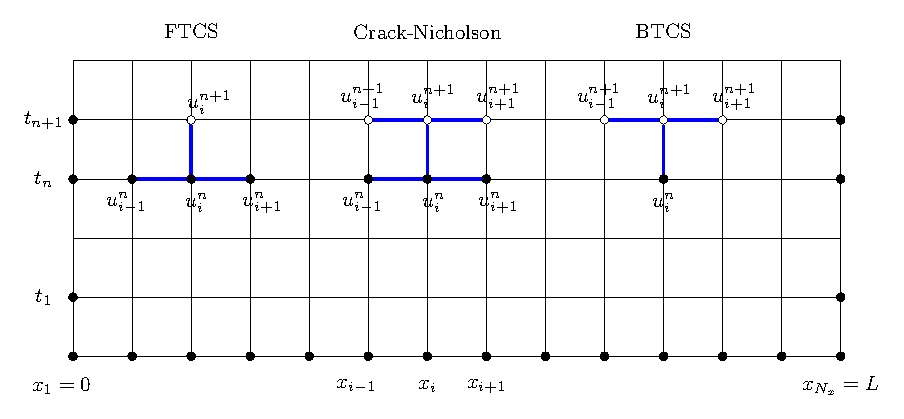
\includegraphics[scale=0.6]{Imagenes/mallaSolucionEDP_05.eps}
	\caption{Configuración de nodos espaciales y temporales para tres métodos de discretización de EDP parabólicas.}
\end{figure}
\end{frame}

\subsection{Método explícito de diferencias finitas}

\begin{frame}
\frametitle{Método explícito de diferencias finitas}
Comenzaremos la discretización para la ecuación de difusión (\ref{eq:ecuacion_13_36}) junto con las CDF (\ref{eq:ecuacion_13_38}) y (\ref{eq:ecuacion_13_39})
\end{frame}
\begin{frame}
\frametitle{Método explícito de diferencias finitas}
Haciendo una malla espacio-temporal regular, caracterizada por los nodos:
\begin{align}
x_{i} &= (i - 1) \; h_{x}, \hspace{1cm} i = 1, 2, \ldots, N_{x} \label{eq:ecuacion_13_40} \\
t_{n} &= n \; h_{t}, \hspace{1.8cm} n = 0, 1, 2, \ldots \label{eq:ecuacion_13_41}
\end{align}
donde $h_{t}$ es el paso temporal y $h_{x}$ representa el paso entre los $N_{x}$ nodos espaciales.
\end{frame}
\begin{frame}
\frametitle{Método explícito de diferencias finitas}
El espaciamiento de los nodos está dado por:
\begin{equation}
h_{x} = \dfrac{L}{N_{x} - 1}
\label{eq:ecuacion_13_42}
\end{equation}
\end{frame}
\begin{frame}
\frametitle{Método explícito de diferencias finitas}
La primera derivada con respecto al tiempo $\partial u / \partial t$ en el nodo espacio - temporal $(x_{i}, t_{n})$ puede obtenerse de una manera directa a partir de la aproximación lineal de la serie de Taylor con respecto a $t$ para la constante $x = x_{i}$
\[ u_{i}^{n + 1} = u_{i}^{n} + h_{t} \; \left( \dfrac{\partial u}{\partial t} \right)_{i,n} + O(h_{t}^{2}) \]
donde $u_{i}^{n} \equiv u(x_{i}, t_{n})$
\end{frame}
\begin{frame}
\frametitle{Método explícito de diferencias finitas}
Separando la derivada temporal, se obtiene el esquema de diferencias hacia adelante:
\begin{equation}
\left( \dfrac{\partial u}{\partial t} \right)_{i,n} = \dfrac{u_{i}^{n + 1} -u_{i}^{n}}{h_{t}} + O(h_{t})
\label{eq:ecuacion_13_43}
\end{equation}
\end{frame}
\begin{frame}
\frametitle{Método explícito de diferencias finitas}
El carácter \enquote{hacia adelante} se da por la presencia de la solución propagada de $t^{n + 1}$ en la expresión de la derivada en $t^{n}$, mientras que el hecho de que el esquema mantenga sólo el primer orden exacto en $h_{t}$ se debe a la división implícita por $h_{t}$.
\end{frame}
\begin{frame}
\frametitle{Método explícito de diferencias finitas}	
Para la segunda derivada espacial en el nodo espacio - temporal $(x_{i}, t_{n})$, podemos usar el esquema de diferencias centrales:
\begin{equation}
\left( \dfrac{\partial^{2} u}{\partial x^{2}} \right)_{i,n} = \dfrac{u_{i + 1}^{n} - 2 \: u_{i}^{n} + u_{i - 1}^{n}}{h_{x}^{2}} + O(h_{x}^{2})
\label{eq:ecuacion_13_44}
\end{equation}
\end{frame}
\begin{frame}
\frametitle{Método explícito de diferencias finitas}
Que involucra sólo la información de $t_{n}$ y de los puntos espaciales ubicados simétricamente alrededor del nodo donde se está calculando la derivada.
\end{frame}
\begin{frame}
\frametitle{Método FTCS}
Sustituyendo las expresiones de diferencias finitas (\ref{eq:ecuacion_13_43}) y (\ref{eq:ecuacion_13_44}) en la ecuación de difusión (\ref{eq:ecuacion_13_36}), se obtiene el \emph{método espacio - temporal hacia adelante} (\textcolor{blue}{Forward Time Central Space FTCS})
\begin{equation}
\dfrac{u_{i}^{n + 1} - u_{i}^{n}}{h_{t}} =  D \; \dfrac{u_{i + 1}^{n} - 2 \: u_{i}^{n} + u_{i - 1}^{n}}{h_{x}^{2}}
\label{eq:ecuacion_13_45}
\end{equation}
\end{frame}
\begin{frame}
\frametitle{Método FTCS}
Que prorporciona una aproximación del orden $O(h_{x}^{2} + h_{t})$ para la ecuación de difusión en el nodo espacio - temporal $(x_{i}, t_{n})$
\end{frame}
\begin{frame}
\frametitle{Método FTCS}
Por lo que podemos expresar la solución propagada en el siguiente paso temporal $t_{n + 1}$ para cada punto interior $x_{i}$ de la malla espacial, sólo en términos de valores previos de tiempo anterior $t_{n}$:
\begin{equation}
u_{i}^{n + 1} = \lambda \: u_{i - 1}^{n} + (1 - 2 \lambda) \: u_{i}^{n} + \lambda \: u_{i + 1}^{n} \hspace{0.5cm} i = 2, 3, \ldots, N_{x} -1
\label{eq:ecuacion_13_46}
\end{equation}
donde
\begin{equation}
\lambda = \dfrac{D \: h_{t}}{h_{x}^{2}}
\label{eq:ecuacion_13_47}
\end{equation}
\end{frame}
\begin{frame}
\frametitle{Método FTCS}
En cuanto a los valores de la solución en la frontera, están fijos por las condiciones de Dirichlet (\ref{eq:ecuacion_13_39}) a lo largo de la propagación y no requieren ningún tratamiento particular:
\begin{equation}
u_{1}^{n + 1} = u_{1}^{n} = u_{0}^{0}, \hspace{1cm} u_{N_{x}}^{n + 1} = u_{N_{x}}^{n} = u_{L}^{0}
\label{eq:ecuacion_13_48}
\end{equation}
\end{frame}
\begin{frame}
\frametitle{Método FTCS}
Puesto que en cada paso del tiempo, los componentes de la solución propagada pueden expresarse independientemente de la ec. (\ref{eq:ecuacion_13_46}), exclusivamente basada en los datos del paso de tiempo previo.
\end{frame}
\begin{frame}
\frametitle{Proceso de propagación}
Se dice que el \textoazul{método FTCS es explícito} si consideramos el proceso de propagación, al re-escribir la ec. (\ref{eq:ecuacion_13_46}) a la ec. (\ref{eq:ecuacion_13_48}) en notación matricial
\begin{equation}
\mathbf{u}^{n + 1} =  \mathbf{B} \cdot \mathbf{u}^{n}, \hspace{1cm} n = 1, 2, \ldots
\label{eq:ecuacion_13_49}
\end{equation}
\end{frame}
\begin{frame}
\frametitle{Proceso de propagación}
La matriz de propagación $\mathbf{B}$ es tridiagonal y el vector $\mathbf{u}^{n}$ recoge los valores de solución de todos los puntos de malla espacial en el paso de tiempo $t_{n}$:
\fontsize{12}{12}\selectfont
\begin{equation}
\mathbf{B} = \begin{bmatrix}
1 & 0 & & & 0 \\
\lambda & 1 - 2 \lambda & \lambda & & & \\
 & \ddots & \ddots & \ddots & \\
 & & \lambda & 1 - 2 \lambda & \lambda \\
 0 & & & 0 & 1
\end{bmatrix},
\hspace{0.3cm}
\mathbf{u}^{n} = 
\begin{bmatrix}
u_{1}^{n} \\
u_{2}^{n} \\
\vdots \\
u_{N_{x} - 1}^{n} \\
u_{N_{x}}^{n} 
\end{bmatrix}
\label{eq:ecuacion_13_50}
\end{equation}
\end{frame}
\begin{frame}
\frametitle{Método FTCS}
Cada componente de la solución propagada $\mathbf{u}^{n+1}$ de manera individual, se obtiene de la multiplicación de la matriz $\mathbf{B}$ con la solución previa del vector $\mathbf{u}^{n}$.
\end{frame}
\subsection{Algoritmo para el método FTCS}
\begin{frame}
\frametitle{Problema de difusión en 1D}
Consideremos la ecuación de difusión en 1D:
\begin{equation}
\dfrac{\partial u}{\partial t} =  D \: \dfrac{\partial^{2} u}{\partial x^{2}} \hspace{1cm} x \in [0, L] \hspace{0.4cm} t > 0
\label{eq:ecuacion_13_51}
\end{equation}
con una constante de difusión sujeta a las CDF de Dirichlet:
\begin{equation}
u(0, t) = u(L, t) = 0 \hspace{1cm} t > 0
\label{eq:ecuacion_13_52}
\end{equation}
\end{frame}
\begin{frame}
\frametitle{Solución inicial y exacta}
Consideremos una solución inicial del tipo:
\begin{equation}
u x, 0) = \sin \left( \dfrac{\pi \: x}{L} \right) \hspace{1cm} x \in [0, L]
\label{eq:ecuacion_13_53}
\end{equation}
\pause
La solución exacta que satisface este problema es:
\begin{equation}
u(x, t) = \exp \left( \dfrac{- \pi \: D \: t}{L^{2}} \right) \: \sin \left( \dfrac{\pi \: x}{L} \right)
\end{equation}
\end{frame}
\begin{frame}
\frametitle{Otros valores}
Consideramos $D = 0.1$ y $L = 1$, la solución se propaga al valor $t_{\text{max}}=6.0$.
\\
\bigskip
El paso temporal es de $h_{t}=1.25 \times 10^{-2}$, el paso espacial es de $h_{x} = 0.05$, por lo que el parámetro de discretización (ec. \ref{eq:ecuacion_13_47}) es $\lambda=0.5$
\end{frame}
\begin{frame}
\frametitle{Algoritmo para el método FTCS}
La rutina \funcionazul{PropagFTCS} resuelve un problema con CDF de Cauchy para la ecuación de difusión (\ref{eq:ecuacion_13_36}), propagando la solución inicial $u_0[ \ ]$ durante el intervalo de tiempo $ht$ de acuerdo con las ecs. (\ref{eq:ecuacion_13_46}) - (\ref{eq:ecuacion_13_48}) obtenidas aplicando el esquema explícito de discretización FTCS.
\end{frame}
\begin{frame}
\frametitle{Algoritmo para el método FTCS}
El coeficiente de difusión constante, el tamaño del paso espacial y el número de nodos se reciben a través de los argumentos $D$, $hx$, $nx$, respectivamente.
\\
La solución propagada se devuelve por medio de la matriz $u[ \ ]$.
\end{frame}
\begin{frame}
\frametitle{Algoritmo para el método FTCS}
Se supone que la secuencia de manejo en el programa principal realiza cualquier procesamiento adicional, sobre todo para liberar la matriz $u[ \ ]$ para un nuevo paso de propagación guardando su contenido en $u0[ \ ]$.
\end{frame}
\begin{frame}
\frametitle{Algoritmo para el método FTCS}
El código primero inicializa la solución $u0[ \ ]$ mediante una llamada a la función \funcionazul{Init} y luego controla la propagación dentro de un bucle temporal mediante llamadas repetidas a \funcionazul{PropagFTCS}, cada una seguida necesariamente por una transferencia hacia atrás del contenido de $u[ \ ]$ a $u0[ \ ]$.    
\end{frame}
{\setbeamercolor{background canvas}{bg=white}
\begin{frame}[fragile]
\frametitle{Propagador explícito FTCS}
\begin{lstlisting}[caption=Propagador explícito FTCS para la ecuación de difusión, style=FormattedNumber, basicstyle=\linespread{1.1}\ttfamily=\small, columns=fullflexible]
def PropagFTCS(u_0_, u, nx, D, hx,ht):

   lam = D*ht/(hx*hx) 
   lam_1_ = 1e0 - 2e0*lam

   u[_1_] = u_0_[_1_]; u[nx] = u_0_[nx]
   for i in range(2, nx):
      u[i] = lam*u_0_[i-_1_]+lam_1_*u_0_[i]+lam*u_0_[i+_1_]
      
   return u
\end{lstlisting}
\end{frame}
\begin{frame}[fragile, allowframebreaks]
\frametitle{Programa principal}
\begin{lstlisting}[caption=Programa principal para el ejercicio, style=FormattedNumber, basicstyle=\linespread{1.1}\ttfamily=\small, columns=fullflexible]
import matplotlib.pyplot as plt
import numpy as np

def Init(u, x, nx):
   global L
   for i in range(1, nx+1):
       u[i] = np.sin(np.pi * x[i]/L)

D = 0.1e0
L = 1e0
nx = 21
tmax = 6.0e0
ht = 1.25e-2

u_0_ = [_0_]*(nx+1); u = [_0_]*(nx+1)

x = [_0_]*(nx+1)

hx = L/(nx-1)

for i in range(1,nx+1):
    x[i] = (i-1)*hx

Init(u_0_, x, nx)

t = 0e0

while (t < tmax):
   t += ht
   PropagFTCS(u_0_, u, nx, D, hx, ht)
   for i in range(1,nx):
       u_0_[i] = u[i]                  

f = np.exp(-np.pi*np.pi*D*t/(L*L))

exacta = []

for i in range(nx+1):
   exacta.append(f * np.sin(np.pi*x[i]/L))

plt.plot(x, u, 'r', label='FTCS', ls='dashed')
plt.plot(x, exacta, 'b', label='Exacta')
plt.title('Solucion numerica para el problema de difusion con $\lambda=0.50$')
plt.xlabel('x')
plt.ylabel('u')
plt.legend(loc=1)
plt.xlim([0,1])
plt.ylim(ymin=0)
plt.show()
\end{lstlisting}
\end{frame}
\begin{frame}
\frametitle{Gráfica del perfil espacial}
\begin{figure}
	\centering
	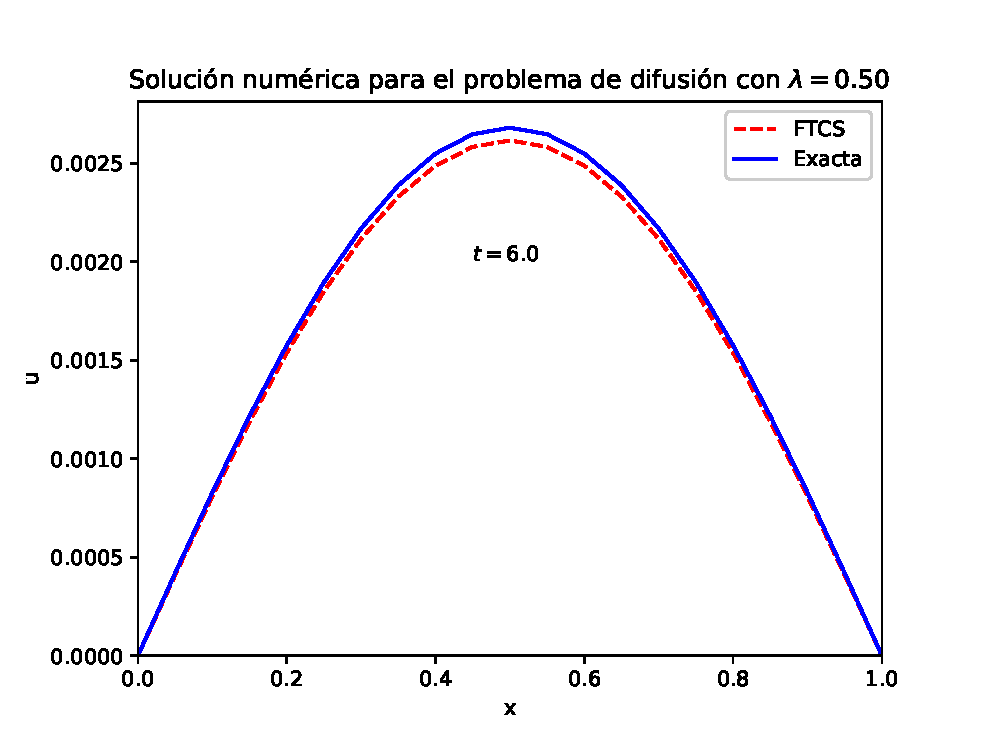
\includegraphics[scale=0.6]{Imagenes/solucionFTSC_01.eps}
\end{figure}
\end{frame}
\begin{frame}
\frametitle{Gráfica de los perfiles a tres tiempos}
\begin{figure}
	\centering
	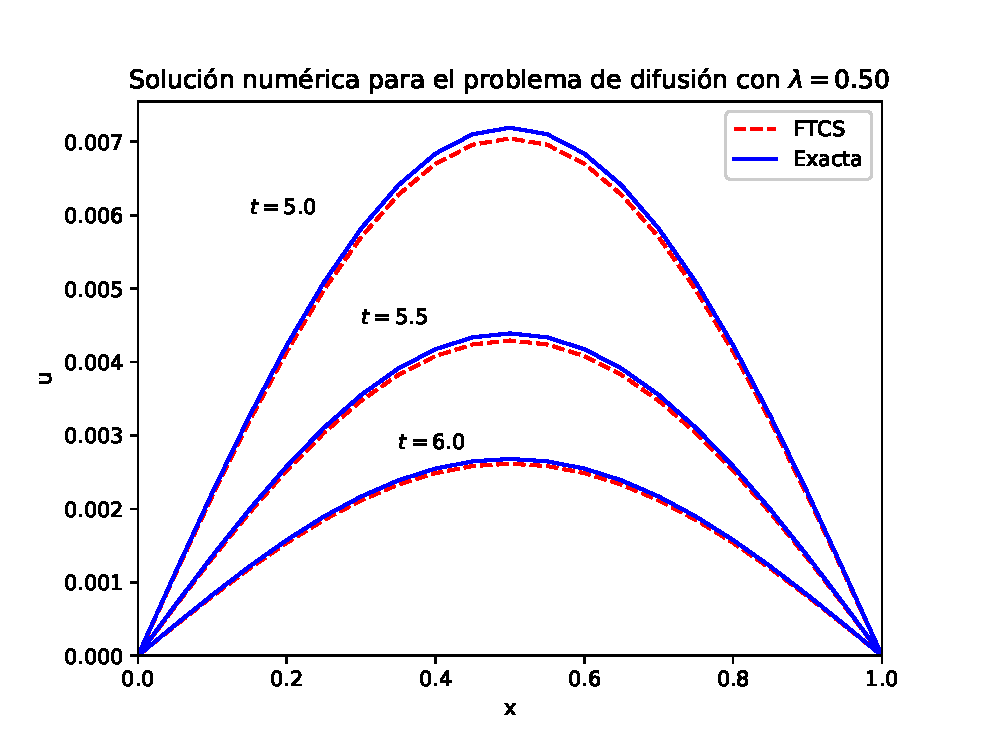
\includegraphics[scale=0.6]{Imagenes/solucionFTSC_02.eps}
\end{figure}
\end{frame}
}
\begin{frame}
\frametitle{Inestabilidad en el método FTCS}
La solución de la ecuación de difusión (\ref{eq:ecuacion_13_36}) por el método explícito FTCS es propensa a una fenomenología numérica particular, siendo confrontada bajo ciertas condiciones con una inestabilidad numérica severa.
\end{frame}
\begin{frame}
\frametitle{Inestabilidad en el método FTCS}
La inestabilidad implica que, en lugar de perfiles espaciales suaves y de buen comportamiento, la propagación desarrolla oscilaciones espúreas, que crecen exponencialmente en el tiempo, distorsionando la solución de manera irrecuperable.
\end{frame}
\begin{frame}
\frametitle{Inestabilidad en el método FTCS}
Este comportamiento crítico se debe al creciente dominio de los errores de redondeo y siempre surge cuando el tamaño del paso de tiempo excede un cierto límite superior, que se correlaciona con el tamaño de paso espacial empleado.
\end{frame}	
\begin{frame}
\frametitle{Cambio en los valores del paso temporal}
Usaremos ahora el valor de $h_{t}=1.30 \times 10^{-2}$, manteniendo el mismo paso espacial de $h_{x}=0.05$.
\\
\bigskip
\pause
El parámetro de discretización ahora será $\lambda=0.52$, ligeramente mayor a $\lambda=0.50$.
\end{frame}
\begin{frame}
\frametitle{Cambio en los valores del paso temporal}
Ocupando el mismo algoritmo de solución, ejecutamos el código y a continuación veremos el comportamiento de la solución.
\end{frame}
{\setbeamercolor{background canvas}{bg=white}
\begin{frame}
\frametitle{Perfiles de solución}
\begin{figure}
	\centering
	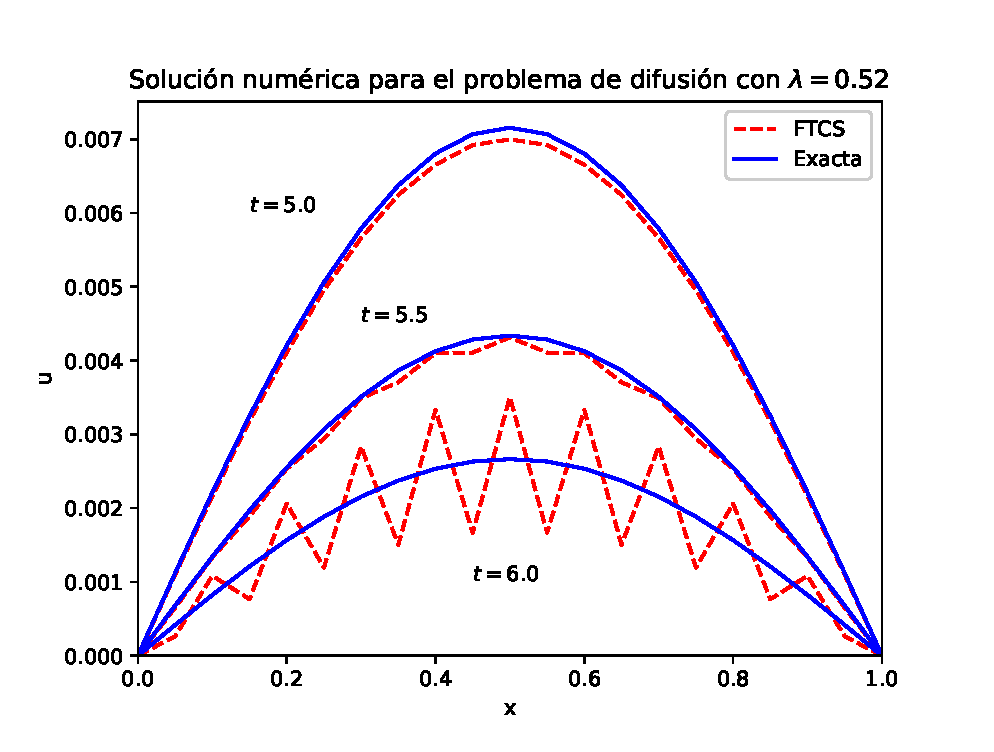
\includegraphics[scale=0.6]{Imagenes/solucionFTSC_03.eps}
\end{figure}
\end{frame}
}
\begin{frame}
\frametitle{Inestabilidad para un valor de $\lambda$}
Mientras que en $t = 5.0$, las soluciones obtenidas con los dos pasos de tiempo son apenas perceptibles, las inestabilidades comienzan a desarrollarse en $t = 5.5$, y dominan completamente la solución en $t = 6.0$.
\end{frame}
\begin{frame}
\frametitle{Inestabilidad para un valor de $\lambda$}
Por lo tanto, un aumento aparentemente marginal del paso de tiempo $h_{t}$ genera un tremendo cambio cualitativo en el comportamiento de la solución.
\end{frame}
\begin{frame}
\frametitle{Inestabilidad para un valor de $\lambda$}
Entonces con $\lambda = 1/2$ se tiene un valor crítico, que separa dos dominios distintos de propagación estable $(\lambda \leq 1/2)$ e inestable $(\lambda > 1/2)$, respectivamente.
\end{frame}
\begin{frame}
\frametitle{Criterio de inestabilidad}
Revisa la guía de apoyo con el tema de análisis de estabilidad de Von Neumann, en donde se desarrolla y discuten ciertas características y propiedades de las soluciones para las EDP con los esquemas mostrados.
\end{frame}

%Referencia Landau - Capítulo 17
\section{Ejercicios}
\frame{\tableofcontents[currentsection, hideothersubsections]}
\subsection{Ecuación de calor}

\begin{frame}
\frametitle{Problema de inicio}
\framesubtitle{Ecuación de calor}
Tenemos una barra de aluminio con una longitud $L = 1 \si\meter$ y de diámetro $w$ (vista desde el eje $x$). La barra está aislada en su perímetro, excepto en los extremos.
\begin{figure}
	\centering
	\includestandalone[scale = 0.6]{ejemploBarraCalor_01}
	\caption{La barra está rodeada de un aislante.}
\end{figure}
\end{frame}
\begin{frame}
\frametitle{Condiciones del problema}
Al inicio, la barra tiene una temperatura uniforme de \SI{100}{\degreeCelsius} y los extremos de la misma están en contacto con agua helada a \SI{0}{\degreeCelsius}. El calor fluye hacia los extremos que no están dentro del aislante.
\begin{figure}
	\centering
	\includestandalone[scale = 0.6]{ejemploBarraCalor_02}
	\caption{Condiciones de temperatura dentro y en los extremos de la barra.}
\end{figure}
\end{frame}
\begin{frame}
\frametitle{¿Qué tenemos que hacer?}
El problema a resolver es el siguiente:
\\
\bigskip
Calcular cómo varía la temperatura a lo largo de la barra conforme trasncurre el tiempo.
\end{frame}
\begin{frame}
\frametitle{Ecuación de calor}
¿Cómo es el flujo de calor de una región caliente a una región fría?
\end{frame}
\begin{frame}
\frametitle{Ecuación de calor}
Expresando el fenómeno en términos matemáticos: decimos que la razón de cambio de flujo de calor $H$ a través de un material, es proporcional al gradiente de temperatura $T$ en el material.
\begin{equation}
H = -K \; \nabla T(x, t)
\label{eq:ecuacion_17_55}	
\end{equation}
donde $K$ es la conductividad térmica del material.
\end{frame}
\begin{frame}
\frametitle{Ecuación de calor}
La cantidad total de calor $Q(t)$ en el material y para cualquier momento, es proporcional a la  integral de la temperatura sobre del volumen del material:
\begin{equation}
Q(t) = \scaleint{6ex} C \: \rho(x) \: T (x, t) \dd{x}
\label{eq:ecuacion_17_56}
\end{equation}
Donde $C$ es el calor específico del material y $\rho$ es la densidad del material. 
\end{frame}
\begin{frame}
\frametitle{Ecuación de calor}
Dado que la energía se conserva, la razón de decremento de $Q$ con el tiempo debe de ser igual a la cantidad de calor fluyendo fuera del material. 
\end{frame}
\begin{frame}
\frametitle{Ecuación de calor}
Después de este balance de energía, aplicamos el teorema de la divergencia, y por tanto la ecuación de calor resulta:
\begin{equation}
\dfrac{\partial T(x,t)}{\partial t} = \dfrac{K}{C \: \rho} \: \nabla^{2} T(x,t)
\label{eq:ecuacion_17_57}
\end{equation}
Suponemos que la densidad del material es constante.
\end{frame}
\begin{frame}
\frametitle{Ecuación de calor}
Tenemos una EDP de tipo parabólico con variables de posición y tiempo independientes. 
\end{frame}
\begin{frame}
\frametitle{Ecuación de calor}
Al especificar este tipo de problema, implica que no hay variación de la temperatura en las direcciones perpendiculares de la barra $(y, z)$, por lo que sólo tenemos una coordenada espacial en el laplaciano:
\begin{equation}
\dfrac{\partial T(x,t)}{\partial t} = \dfrac{K}{C \: \rho} \: \dfrac{\partial^{2} T(x, t)}{\partial x^{2}}
\label{eq:ecuacion_17_58}
\end{equation}
\end{frame}
\begin{frame}
\frametitle{Ecuación de calor}
La temperatura inicial de la barra y las condiciones de frontera son:
\begin{align}
\begin{aligned}
T(x, t=0) &= \SI{100}{\degreeCelsius} \\
T(x=0, t) = T(x=L, t) &= \SI{0}{\degreeCelsius}
\end{aligned}
\label{eq:ecuacion_17_59}
\end{align}
\end{frame}
\subsection{Solución numérica}
\begin{frame}
\frametitle{Solución numérica}
Como se revisó con la ecuación de Laplace y con la de difusión, la solución numérica se basa en convertir una ecuación diferencial en una aproximación por diferencias finitas.
\\
\bigskip
Se discretiza el espacio y el tiempo en una malla y se resuelven las soluciones en los nodos.
\end{frame}
\begin{frame}
\frametitle{Malla para los cálculos}
\begin{figure}
	\centering
	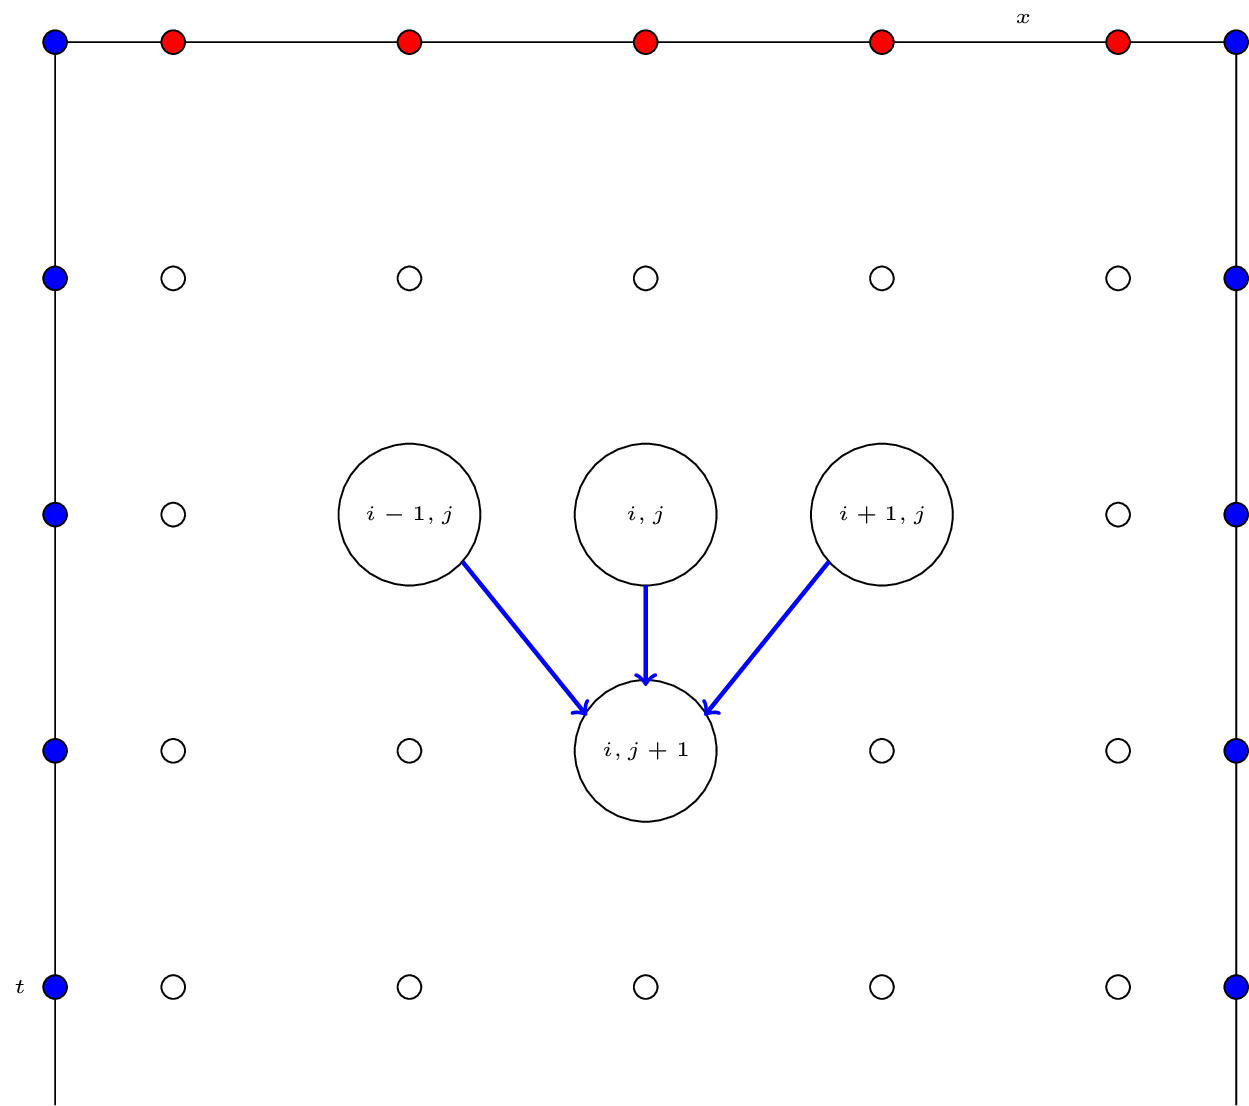
\includegraphics[scale=0.15]{Imagenes/malla_parabolica_01.png}
\end{figure}
\end{frame}
\begin{frame}
\frametitle{Solución numérica}
Los nodos horizontales de color rojo corresponden a los valores conocidos de la temperatura para el tiempo inicial, mientras que los nodos azules verticales corresponden a la temperatura fija en los extremos.
\end{frame}
\begin{frame}
\frametitle{Solución numérica}
Con sólo la fila superior conocida, proponemos un algoritmo que avanza en el tiempo una fila a la vez, como en el salto de una rana, a este método se le conoce como \textocolor{ao}{leapfrog}.
\end{frame}
\begin{frame}
\frametitle{Desarrollo para la solución}
Como suele ser el caso con EDP, el algoritmo se personaliza para la ecuación que se está resolviendo y para las restricciones impuestas por el conjunto particular de condiciones iniciales y de frontera.
\end{frame}
\begin{frame}
\frametitle{Primera derivada para la solución}
Con solo un renglón de datos para comenzar, usamos una aproximación por diferencias hacia adelante para la derivada de la temperatura con respecto al tiempo
\begin{equation}
\dfrac{\partial T(x,t)}{\partial t} \simeq \dfrac{T(x, t + \Delta t) - T(x, t)}{\Delta t}
\label{eq:ecuacion_17_68}
\end{equation}
\end{frame}
\begin{frame}
\frametitle{Primera derivada para la solución}
Debido a que conocemos la variación espacial de la temperatura a lo largo de toda la fila superior y en los lados izquierdo y derecho, estamos menos limitados con la derivada espacial que con la derivada del tiempo.
\end{frame}
\begin{frame}
\frametitle{Segunda derivada para la solución}
Usaremos una aproximación por diferencias central para la derivada espacial
\begin{equation}
\dfrac{\partial^{2} T(x,t)}{\partial x^{2}} \simeq \dfrac{T(x + \Delta x, t ) - T(x - \Delta x, t) - 2 \: T(x,t)}{(\Delta x)^{2}}
\label{eq:ecuacion_17_69}
\end{equation}
\end{frame}
\begin{frame}
\frametitle{Ecuacion por diferencias finitas}
Al sustituir las aproximaciones en la ec. (\ref{eq:ecuacion_17_58}), se obtiene la ecuación de calor por diferencias:
\begin{align}
\begin{aligned}
& \dfrac{K}{C \: \rho} \: \dfrac{T(x + \Delta x, t) - T(x - \Delta x, t) - 2 \: T(x,t)}{(\Delta x)^{2}}
\end{aligned}
\label{eq:ecuacion_17_70}
\end{align}
\end{frame}
\begin{frame}
\frametitle{Algoritmo discretizado}
Reordenamos la ec. (\ref{eq:ecuacion_17_70}) en una forma en la que $T$ puede avanzar en $t$:
\begin{equation}
T_{i, j+1} = T_{i, j} + \eta \left[ T_{i+1, j} + T_{i-1, j} - 2 \: T_{i, j} \right], \hspace{0.5cm} \eta = \dfrac{K \: \Delta t}{C \: \rho \: \Delta x^{2}}
\label{eq:ecuacion_17_71}
\end{equation}
donde $x = i \: \Delta x $ y $t = j \: \Delta t$.
\end{frame}
\begin{frame}
\frametitle{Naturaleza del algoritmo}
Este algoritmo es \textocolor{ao}{explícito} porque proporciona una solución en términos de valores conocidos de la temperatura.
\end{frame}
\begin{frame}
\frametitle{Naturaleza del algoritmo}
Si tratamos de resolver simultáneamente la temperatura en todos los sitios de la malla, entonces tendríamos un algoritmo \textocolor{red}{implícito} que requiere que resolvamos las ecuaciones que involucran valores desconocidos de la temperatura.
\end{frame}
\begin{frame}
\frametitle{Naturaleza del algoritmo}
Vemos que la temperatura en el nodo espacio-tiempo $(i, j+1)$ se calcula a partir de los tres valores de temperatura en un tiempo anterior $j$ y en los valores espaciales adyacentes $i \pm 1, i$.
\end{frame}
\begin{frame}
\frametitle{Naturaleza del algoritmo}
Comenzamos la solución en la fila superior, avanzando en el tiempo y manteniendo la temperatura a lo largo de los extremos fijos en $0 \si\celsius$.
\end{frame}
\subsection{Resolviendo el problema}
\begin{frame}
\frametitle{Datos para el problema}
Considera una barra de aluminio de longitud $L = 1 \si\meter$, con las condiciones de frontera y condiciones iniciales:
\begin{align}
\begin{aligned}
T(x = 0, t) = T(x = L, t) &= \SI{0}{\degreeCelsius} \\
T(x, t = 0) &= \SI{100}{\degreeCelsius}
\end{aligned}
\label{eq:ecuacion_17_77}
\end{align}
\end{frame}
\begin{frame}[fragile]
\frametitle{Datos para el problema}
La conductividad térmica, el calor específico y la densidad del aluminio son, respectivamente:
\begin{align}
\begin{aligned}
K &= 237 \: \si{\watt\per\meter\per\kelvin} \\
C &= 900 \: \si{\joule\per\kilogram\per\kelvin} \\
\rho &= 2700 \: \si{\kilogram\per\cubic\metre}
\end{aligned}
\label{eq:ecuacion_17_78}
\end{align}
\end{frame}
{\setbeamercolor{background canvas}{bg=white}
\begin{frame}[plain, fragile]
\frametitle{Importando las librerías}
\begin{lstlisting}[caption=Llamada a las librerías, style=FormattedNumber, basicstyle=\linespread{1.1}\ttfamily=\small, columns=fullflexible]
import numpy as np
import matplotlib.pyplot as plt
from mpl_\textunderscore_toolkits.mplot_3_d import Axes_3_D
from matplotlib import cm
\end{lstlisting}
\end{frame}
\begin{frame}
\frametitle{Declarando valores}
Se declaran las constantes físicas del aluminio, así como dos los valores: $Nx$ para los puntos en la barra y $Nt$ para la evolución temporal, así como el incremento espacial $\Delta x = 0.01414$ y el incremento temporal $\Delta t= 1$.
\end{frame}
\begin{frame}[allowframebreaks, plain, fragile]
\frametitle{Declarando valores}
\begin{lstlisting}[caption=Declarando valores para el algoritmo, style=FormattedNumber, basicstyle=\linespread{1.1}\ttfamily=\small, columns=fullflexible]
kappa = 210.
sph = 900.
rho = 2700.
Nx = 101
Nt = 3000
Dx = 0.01414
Dt = 1.

cons = kappa/(sph*rho)*Dt/(Dx*Dx)
\end{lstlisting}
\end{frame}
\begin{frame}[allowframebreaks, plain, fragile]
\frametitle{Arreglos para los cálculos}
Se generan los arreglos para almacenar los valores nuevos de temperatura y de tiempo:
\begin{lstlisting}[caption=Arreglos para los cálculos de temperatura, style=FormattedNumber, basicstyle=\linespread{1.1}\ttfamily=\small, columns=fullflexible]
T = np.zeros((Nx, 2), dtype=float)
Tpl = np.zeros ((Nx, 31), dtype=float)
\end{lstlisting}
\end{frame}
\begin{frame}[allowframebreaks, plain, fragile]
\frametitle{Condiciones iniciales y de frontera}
Se establecen las condiciones iniciales y de frontera:
\begin{lstlisting}[caption=Se definen las condiciones iniciales y de frontera, style=FormattedNumber, basicstyle=\linespread{1.1}\ttfamily=\small, columns=fullflexible]
for ix in range(1, Nx-1):
    T[ix, _0_] = 100.0

T[_0_, _0_] = 0.0
T[_0_, _1_] = 0.0

T[Nx-_1_, _0_] = 0.0
T[Nx-_1_, _1_] = 0.0
\end{lstlisting}
\end{frame}
\begin{frame}[plain, allowframebreaks, fragile]
\frametitle{Ciclo de iteración}
\begin{lstlisting}[caption=Ciclo de iteración para calcular los nuevos valores de temperatura, style=FormattedNumber, basicstyle=\linespread{1.1}\ttfamily=\small, columns=fullflexible]
m = 1

for t in range(1, Nt):
    for ix in range(1, Nx-1):
        T[ix, _1_] = T[ix,_0_]+cons*(T[ix+_1_,_0_]+T[ix-_1_,_0_]-2.*T[ix,_0_])
    if t%100 == 0 or t == 1:
        for ix in range(1,Nx-_1_,2):
            Tpl[ix,m] = T[ix,_1_]
        print (m)
        m = m+1
    for ix in range(1, Nx-1):
        T[ix,_0_] = T[ix,_1_]
\end{lstlisting}
\end{frame}
\begin{frame}[plain, allowframebreaks, fragile]
\frametitle{Creando la malla para la solución}
Se crea la malla espacio-temporal y definimos una función que nos devuelve la temperatura
\begin{lstlisting}[caption=Definición de la malla, style=FormattedNumber, basicstyle=\linespread{1.1}\ttfamily=\small, columns=fullflexible]
x = list(range(1, Nx-1, 2))
y = list(range(1, 30))

X, Y = np.meshgrid(x,y)

def functz(Tpl):
    z = Tpl[X,Y]
    return z
    
Z = functz(Tpl)
\end{lstlisting}
\end{frame}
\begin{frame}[plain, allowframebreaks, fragile]
\frametitle{Graficando los resultados}
Hacemos la rutina para presentar los datos en una gráfica 3D con \funcionazul{matplotlib}
\begin{lstlisting}[caption=Rutina para graficar los resultados, style=FormattedNumber, basicstyle=\linespread{1.1}\ttfamily=\small, columns=fullflexible]
fig = plt.figure()
ax = fig.add_subplot(projection='3d')

surf = ax.plot_\textunderscore_surface(X,Y,Z,rstride=1,cstride=1,linewidth=0.5,cmap=cm.hot_\textunderscore_r)

ax.set_\textunderscore_zlim(-50, 100)

cset = ax.contourf(X,Y,Z,zdir='z',offset=-50,cmap=cm.hot_\textunderscore_r)
cbar = fig.colorbar(surf,shrink=0.5,aspect=5)
cbar.ax.set_\textunderscore_ylabel('Temperatura',rotation=270,labelpad=10)
ax.set_\textunderscore_xlabel('Posicion')
ax.set_\textunderscore_ylabel('Tiempo')
plt.title('Grafica obtenida con el algoritmo para la ecuacion de calor')
plt.show()
\end{lstlisting}
\end{frame}
\begin{frame}
\frametitle{Gráfica obtenida}
\begin{figure}
	\centering
	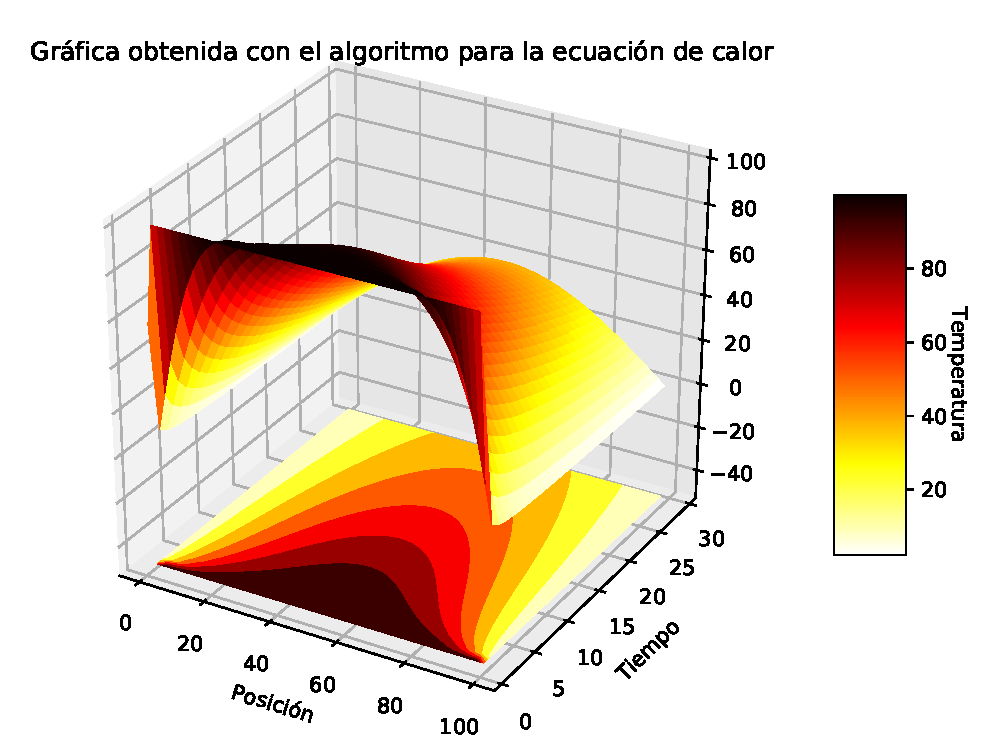
\includegraphics[scale=0.55]{Imagenes/SolucionEcuacionCalor_01.eps}  
\end{figure}
\end{frame}
}

\section{Problemas a resolver a cuenta de examen}
\frame{\tableofcontents[currentsection, hideothersubsections]}
\subsection{Ejercicios}

\begin{frame}
\frametitle{Problemas a resolver}
Se hacen algunos cambios en el planteamiento del problema, pero el algoritmo que hay que usar es el mismo, hay que resolver los siguientes casos:
\setbeamercolor{item projected}{bg=bole,fg=white}
\setbeamertemplate{enumerate items}{%
\usebeamercolor[bg]{item projected}%
\raisebox{1.5pt}{\colorbox{bg}{\color{fg}\footnotesize\insertenumlabel}}%
}
\begin{enumerate}[<+->]
\item Distribución inicial de temperatura de forma senoidal: $\sin( \pi x / L)$
\item Dos barras en contacto cada una con diferente temperatura.
\item Modificación de la ecuación de calor para incluir un término y obtener la ley de enfriamiento de Newton.
\end{enumerate}
\end{frame}

\subsection{Problema 1}

\begin{frame}
\frametitle{Problema 1}
Distribución inicial de temperatura de forma senoidal: $\sin( \pi x / L)$
\\
\bigskip
Utiliza las mismas constantes que en el primer ejemplo. Puedes comparar los resultados con la solución analítica:
\[ T(x,t) = \sin \left( \dfrac{\pi \: x}{L} \right) \: \exp \left(-\dfrac{\pi^{2} \: R \: t}{L^{2}} \right), \hspace{0.75cm} R=\dfrac{K}{C \: \rho} \]
\end{frame}
\begin{frame}
\frametitle{Solución del problema 1}
\begin{figure}
	\centering
	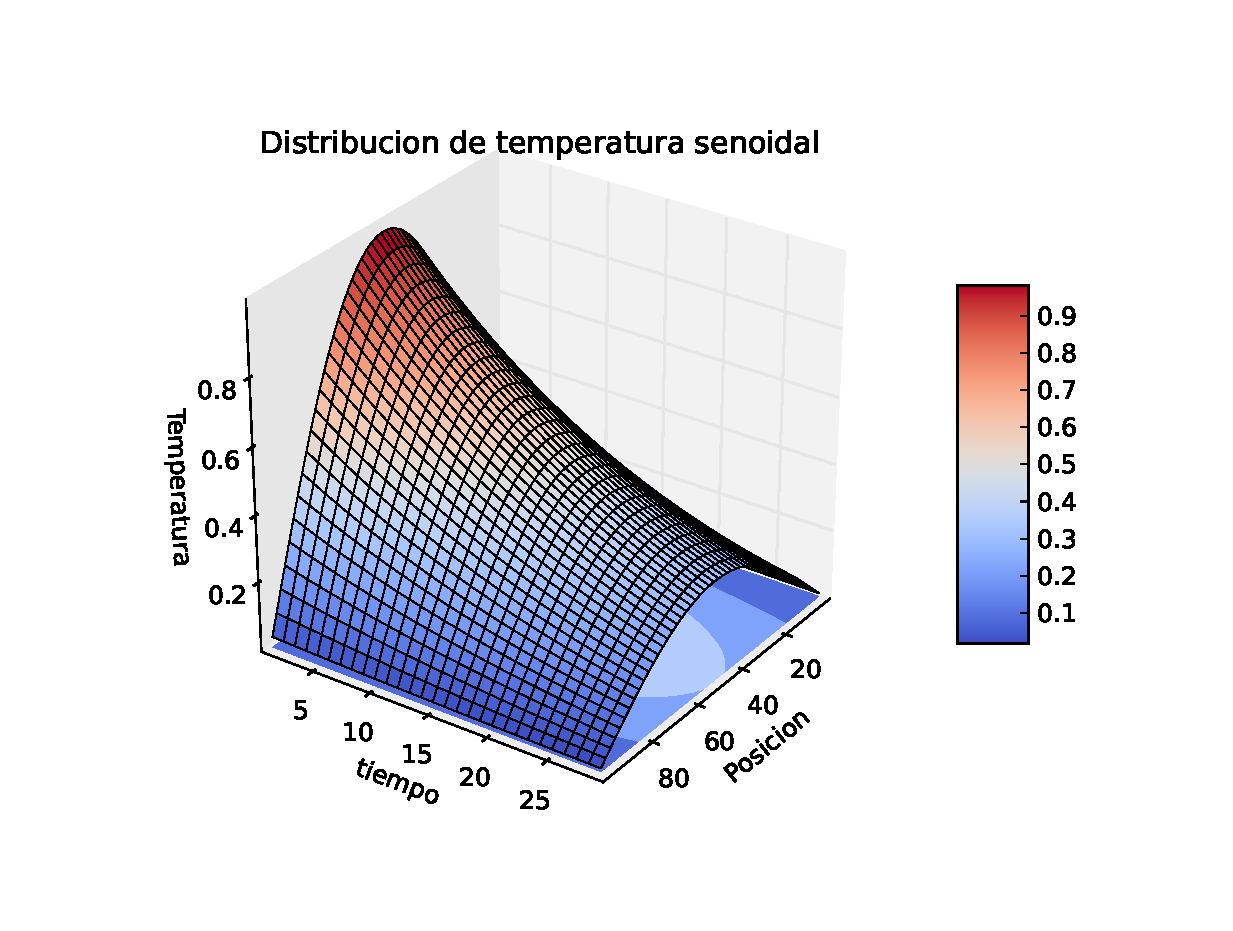
\includegraphics[scale=0.5]{Imagenes/EqCalor04.eps}  
\end{figure}
\end{frame}
\begin{frame}
\frametitle{Solución del problema 1 -rotada-}
\begin{figure}
	\centering
	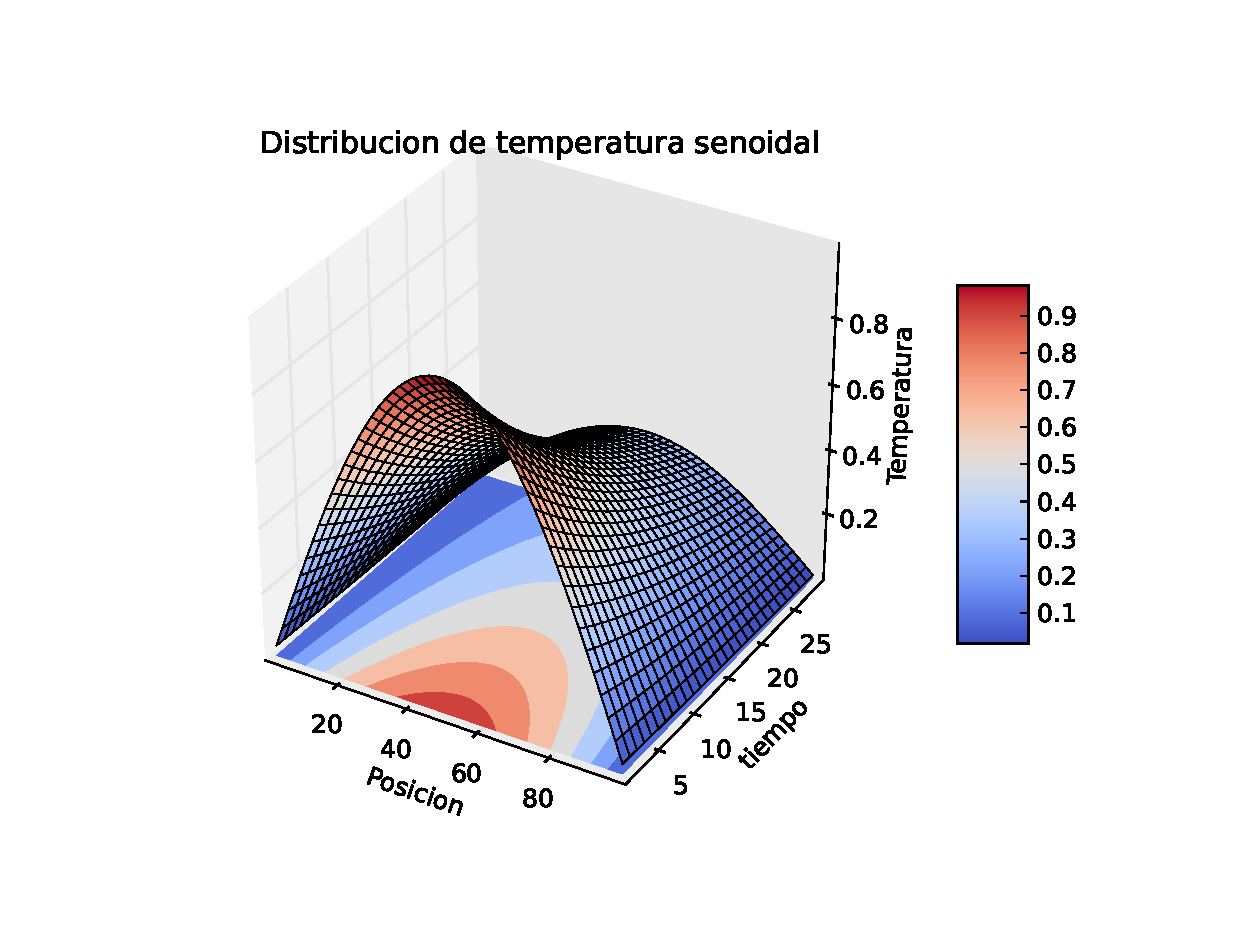
\includegraphics[scale=0.5]{Imagenes/EqCalor05.eps}  
\end{figure}
\end{frame}

\subsection{Problema 2}

\begin{frame}
\frametitle{Problema 2}
Tenemos dos barras del mismo material en contacto, cada una de ellas a diferente temperatura.
\end{frame}
\begin{frame}
\frametitle{Problema 2}
Las barras miden  $50 \: \si\cm$ de longitud. Una de ellas se mantiene a una temperatura de $100 \: \si\celsius$ y la otra a $50 \si\celsius$, se ponen en contacto a lo largo de su eje, un extremo de cada barra se mantiene a $0 \: \si\celsius$.
\\
\bigskip
Determina cómo varía la temperatura con respecto a la posición y al tiempo.
\end{frame}
\begin{frame}
\frametitle{Dos barras con diferente temperatura en contacto}
\begin{figure}
	\centering
	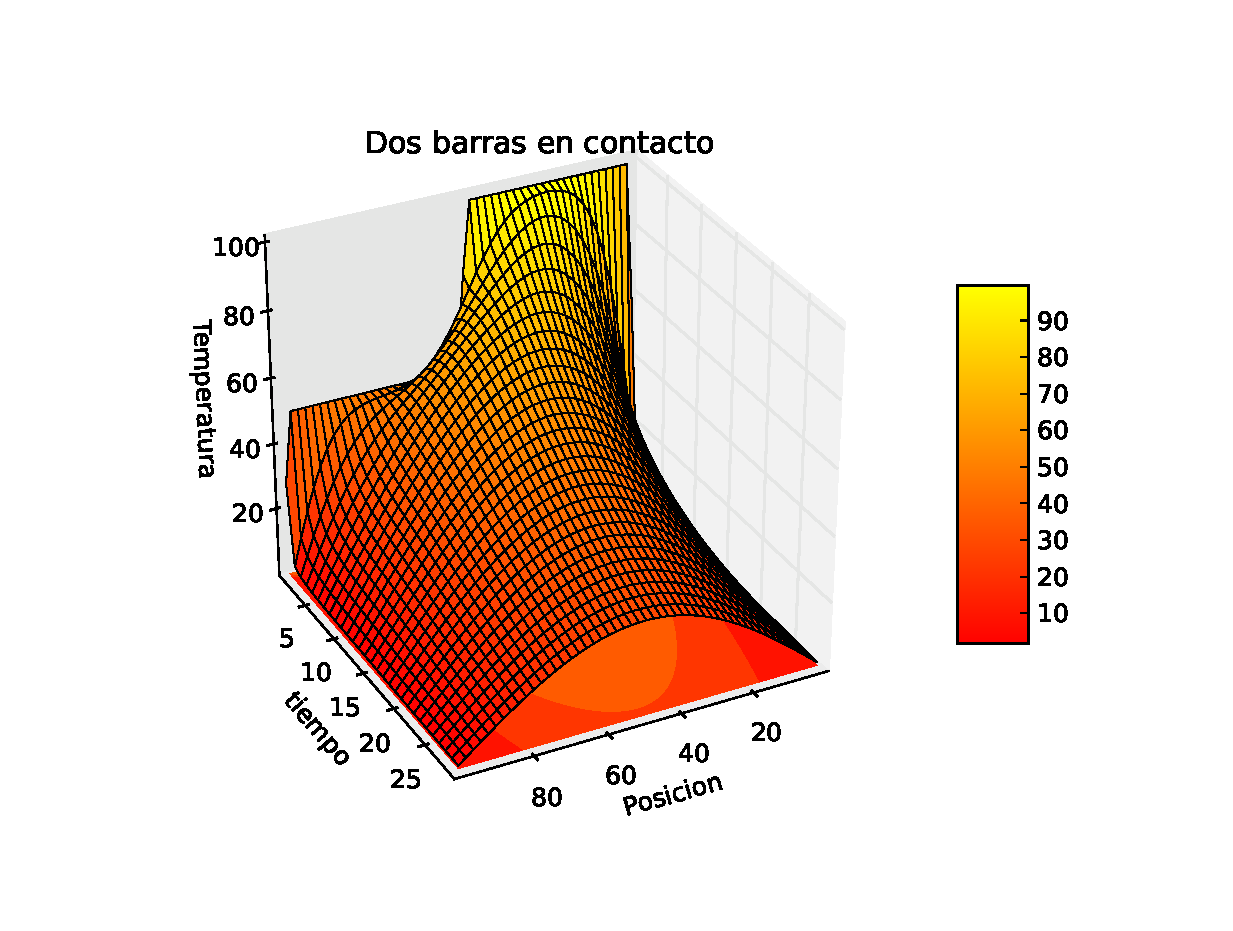
\includegraphics[scale=0.5]{Imagenes/EqCalor06.eps}  
\end{figure}
\end{frame}
\begin{frame}
\frametitle{Dos barras en contacto -rotada-}
\begin{figure}
	\centering
	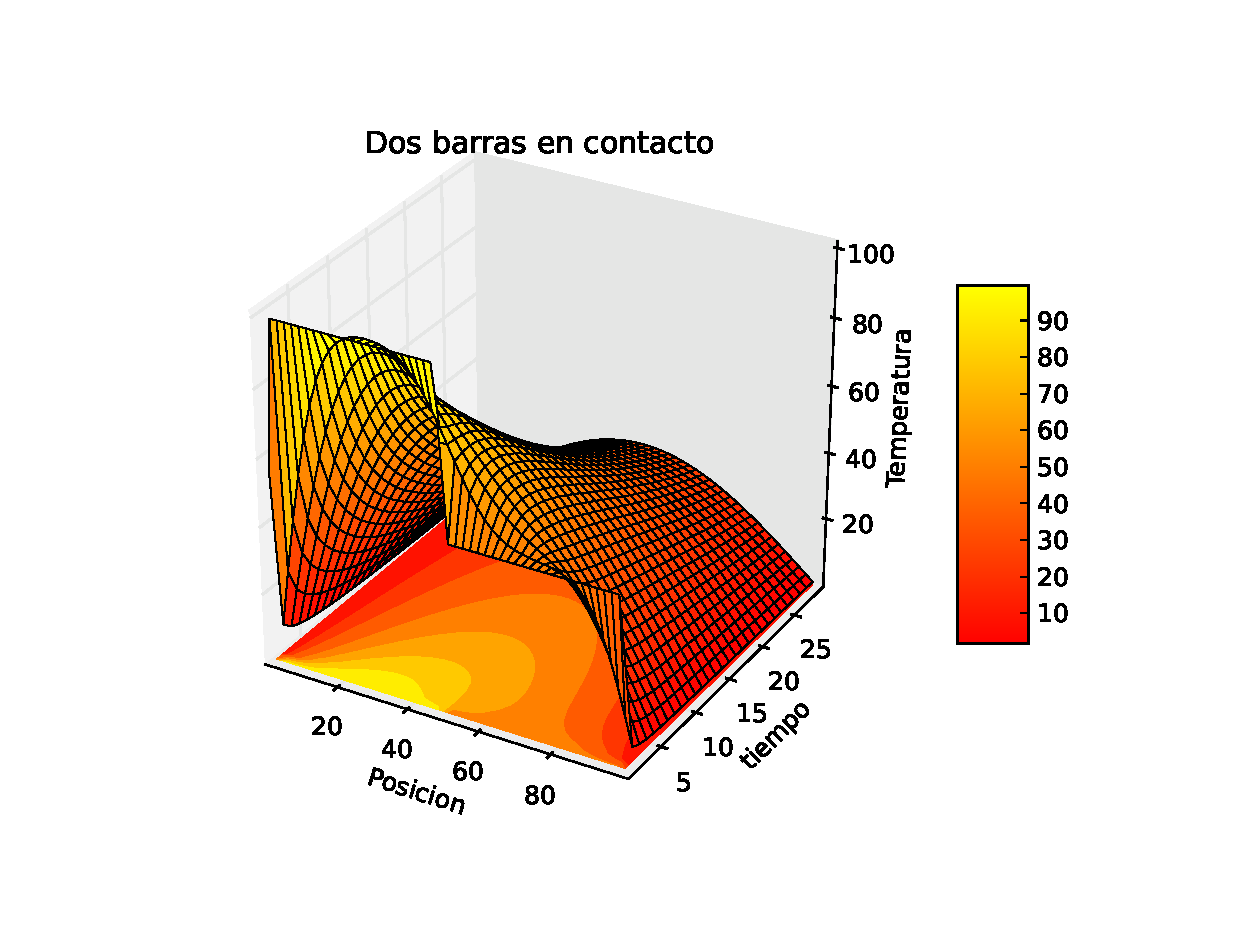
\includegraphics[scale=0.5]{Imagenes/EqCalor07.eps}  
\end{figure}
\end{frame}

\subsection{Problema 3}

\begin{frame}
\frametitle{Problema 3}
Modificación de la ecuación de calor para incluir un término y obtener la ley de enfriamiento de Newton.
\end{frame}
\begin{frame}
\frametitle{Problema 3}
Imagina ahora que la barra que estaba aislada (el problema con el que comenzamos la clase), se deja en contacto con el ambiente que se encuentra a una temperatura $T_{e}$, tal que es diferente a la temperatura inicial de la barra.
\end{frame}
\begin{frame}
\frametitle{Problema 3}
La ley de enfriamiento de Newton nos dice que la razón de cambio de la temperatura debido a la radiación es:
\[ \dfrac{\partial T}{\partial t} = - h (T- T_{e}) \]
\end{frame}
\begin{frame}
La ecuación de calor se modifica, quedando:
\[ \dfrac{\partial T(x,t)}{\partial t} = \dfrac{K}{C \: \rho} \dfrac{\partial^{2}T}{\partial x^{2}} - h \: T(x,t)\]
Ajusta el algoritmo y el programa para introducir el término de enfriamiento de Newton a lo largo de la barra. Compara el enfriamiento de esta barra con el ejemplo de la barra aislada.
\end{frame}
\begin{frame}
\frametitle{Barra aislada}
\begin{figure}
	\centering
	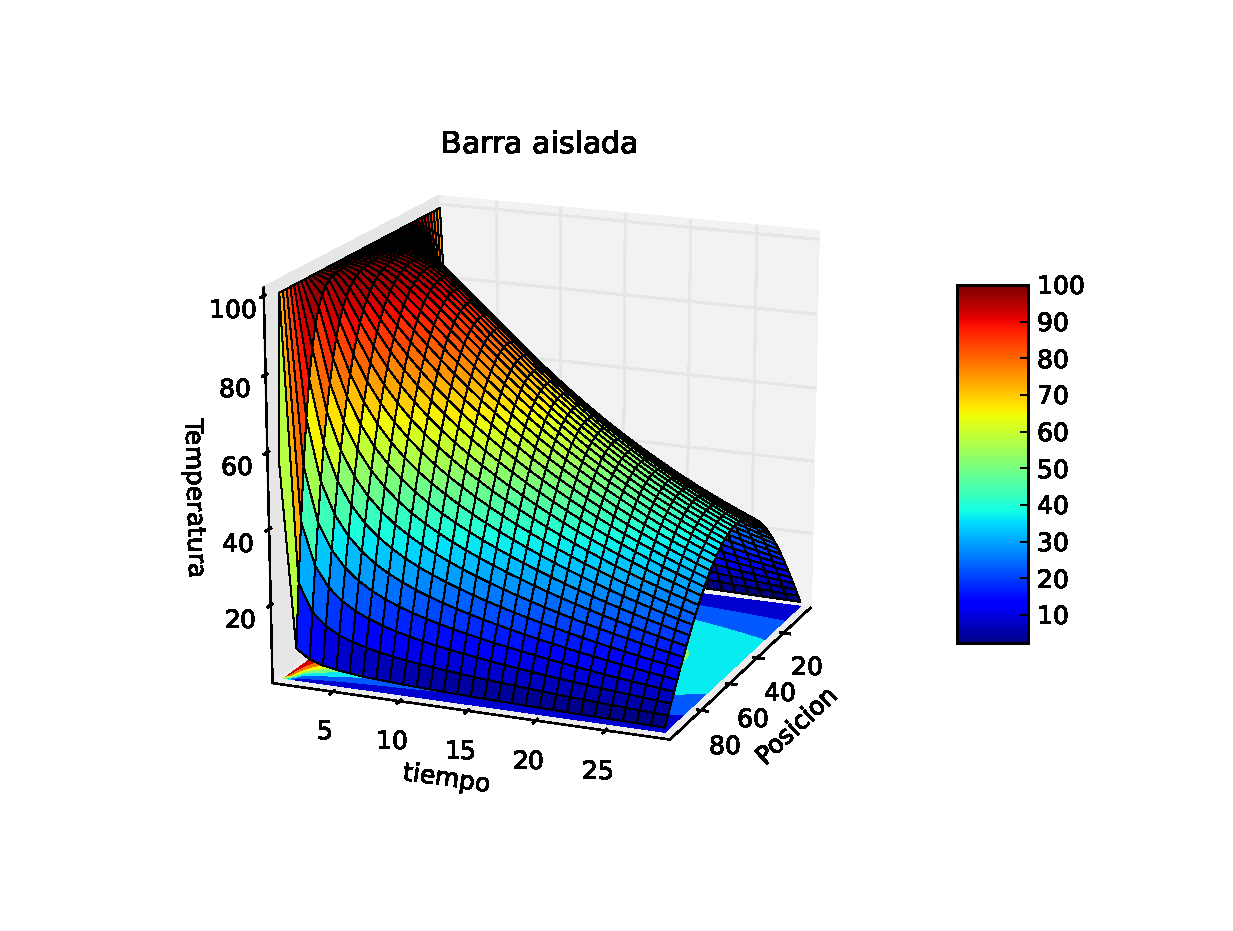
\includegraphics[scale=0.5]{Imagenes/EqCalor08.eps}  
\end{figure}
\end{frame}
\begin{frame}
\frametitle{Ley de enfriamiento de Newton, con $T_{e}=25 \si\celsius$}
\begin{figure}
	\centering
	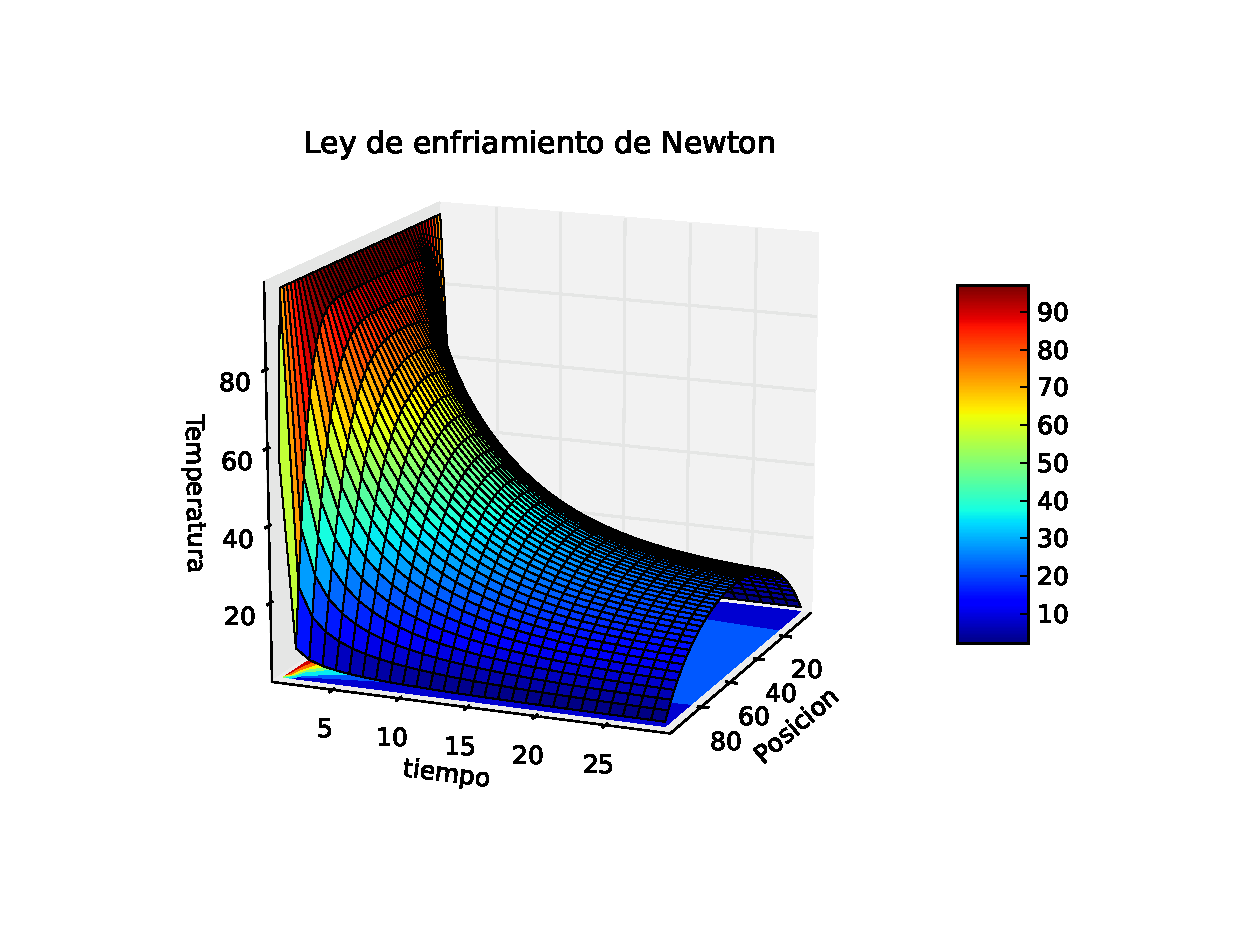
\includegraphics[scale=0.5]{Imagenes/EqCalor09.eps}  
\end{figure}
\end{frame}

\end{document}